% Options for packages loaded elsewhere
\PassOptionsToPackage{unicode}{hyperref}
\PassOptionsToPackage{hyphens}{url}
%
\documentclass[
  english,
  man]{apa6}
\title{DateLife: leveraging databases and analytical tools to reveal the dated Tree of Life}
\author{Luna L. Sánchez Reyes\textsuperscript{1,2}, Emily Jane McTavish\textsuperscript{1}, \& Brian O'Meara\textsuperscript{2}}
\date{}

\usepackage{amsmath,amssymb}
\usepackage{lmodern}
\usepackage{iftex}
\ifPDFTeX
  \usepackage[T1]{fontenc}
  \usepackage[utf8]{inputenc}
  \usepackage{textcomp} % provide euro and other symbols
\else % if luatex or xetex
  \usepackage{unicode-math}
  \defaultfontfeatures{Scale=MatchLowercase}
  \defaultfontfeatures[\rmfamily]{Ligatures=TeX,Scale=1}
\fi
% Use upquote if available, for straight quotes in verbatim environments
\IfFileExists{upquote.sty}{\usepackage{upquote}}{}
\IfFileExists{microtype.sty}{% use microtype if available
  \usepackage[]{microtype}
  \UseMicrotypeSet[protrusion]{basicmath} % disable protrusion for tt fonts
}{}
\makeatletter
\@ifundefined{KOMAClassName}{% if non-KOMA class
  \IfFileExists{parskip.sty}{%
    \usepackage{parskip}
  }{% else
    \setlength{\parindent}{0pt}
    \setlength{\parskip}{6pt plus 2pt minus 1pt}}
}{% if KOMA class
  \KOMAoptions{parskip=half}}
\makeatother
\usepackage{xcolor}
\IfFileExists{xurl.sty}{\usepackage{xurl}}{} % add URL line breaks if available
\IfFileExists{bookmark.sty}{\usepackage{bookmark}}{\usepackage{hyperref}}
\hypersetup{
  pdftitle={DateLife: leveraging databases and analytical tools to reveal the dated Tree of Life},
  pdfauthor={Luna L. Sánchez Reyes1,2, Emily Jane McTavish1, \& Brian O'Meara2},
  pdflang={en-EN},
  pdfkeywords={Tree; Phylogeny; Scaling; Dating; Ages; Divergence times; Open Science; Congruification; Supertree; Calibrations; Secondary calibrations},
  hidelinks,
  pdfcreator={LaTeX via pandoc}}
\urlstyle{same} % disable monospaced font for URLs
\usepackage{graphicx}
\makeatletter
\def\maxwidth{\ifdim\Gin@nat@width>\linewidth\linewidth\else\Gin@nat@width\fi}
\def\maxheight{\ifdim\Gin@nat@height>\textheight\textheight\else\Gin@nat@height\fi}
\makeatother
% Scale images if necessary, so that they will not overflow the page
% margins by default, and it is still possible to overwrite the defaults
% using explicit options in \includegraphics[width, height, ...]{}
\setkeys{Gin}{width=\maxwidth,height=\maxheight,keepaspectratio}
% Set default figure placement to htbp
\makeatletter
\def\fps@figure{htbp}
\makeatother
\setlength{\emergencystretch}{3em} % prevent overfull lines
\providecommand{\tightlist}{%
  \setlength{\itemsep}{0pt}\setlength{\parskip}{0pt}}
\setcounter{secnumdepth}{-\maxdimen} % remove section numbering
% Make \paragraph and \subparagraph free-standing
\ifx\paragraph\undefined\else
  \let\oldparagraph\paragraph
  \renewcommand{\paragraph}[1]{\oldparagraph{#1}\mbox{}}
\fi
\ifx\subparagraph\undefined\else
  \let\oldsubparagraph\subparagraph
  \renewcommand{\subparagraph}[1]{\oldsubparagraph{#1}\mbox{}}
\fi
\newlength{\cslhangindent}
\setlength{\cslhangindent}{1.5em}
\newlength{\csllabelwidth}
\setlength{\csllabelwidth}{3em}
\newlength{\cslentryspacingunit} % times entry-spacing
\setlength{\cslentryspacingunit}{\parskip}
\newenvironment{CSLReferences}[2] % #1 hanging-ident, #2 entry spacing
 {% don't indent paragraphs
  \setlength{\parindent}{0pt}
  % turn on hanging indent if param 1 is 1
  \ifodd #1
  \let\oldpar\par
  \def\par{\hangindent=\cslhangindent\oldpar}
  \fi
  % set entry spacing
  \setlength{\parskip}{#2\cslentryspacingunit}
 }%
 {}
\usepackage{calc}
\newcommand{\CSLBlock}[1]{#1\hfill\break}
\newcommand{\CSLLeftMargin}[1]{\parbox[t]{\csllabelwidth}{#1}}
\newcommand{\CSLRightInline}[1]{\parbox[t]{\linewidth - \csllabelwidth}{#1}\break}
\newcommand{\CSLIndent}[1]{\hspace{\cslhangindent}#1}
\DeclareUnicodeCharacter{0301}{*************************************}
% Manuscript styling
\usepackage{upgreek}
\captionsetup{font=singlespacing,justification=justified}

% Table formatting
\usepackage{longtable}
\usepackage{lscape}
% \usepackage[counterclockwise]{rotating}   % Landscape page setup for large tables
\usepackage{multirow}		% Table styling
\usepackage{tabularx}		% Control Column width
\usepackage[flushleft]{threeparttable}	% Allows for three part tables with a specified notes section
\usepackage{threeparttablex}            % Lets threeparttable work with longtable

% Create new environments so endfloat can handle them
% \newenvironment{ltable}
%   {\begin{landscape}\centering\begin{threeparttable}}
%   {\end{threeparttable}\end{landscape}}
\newenvironment{lltable}{\begin{landscape}\centering\begin{ThreePartTable}}{\end{ThreePartTable}\end{landscape}}

% Enables adjusting longtable caption width to table width
% Solution found at http://golatex.de/longtable-mit-caption-so-breit-wie-die-tabelle-t15767.html
\makeatletter
\newcommand\LastLTentrywidth{1em}
\newlength\longtablewidth
\setlength{\longtablewidth}{1in}
\newcommand{\getlongtablewidth}{\begingroup \ifcsname LT@\roman{LT@tables}\endcsname \global\longtablewidth=0pt \renewcommand{\LT@entry}[2]{\global\advance\longtablewidth by ##2\relax\gdef\LastLTentrywidth{##2}}\@nameuse{LT@\roman{LT@tables}} \fi \endgroup}

% \setlength{\parindent}{0.5in}
% \setlength{\parskip}{0pt plus 0pt minus 0pt}

% \usepackage{etoolbox}
\makeatletter
\patchcmd{\HyOrg@maketitle}
  {\section{\normalfont\normalsize\abstractname}}
  {\section*{\normalfont\normalsize\abstractname}}
  {}{\typeout{Failed to patch abstract.}}
\patchcmd{\HyOrg@maketitle}
  {\section{\protect\normalfont{\@title}}}
  {\section*{\protect\normalfont{\@title}}}
  {}{\typeout{Failed to patch title.}}
\makeatother
\shorttitle{DateLife: revealing the dated Tree of Life}
\keywords{Tree; Phylogeny; Scaling; Dating; Ages; Divergence times; Open Science; Congruification; Supertree; Calibrations; Secondary calibrations\newline\indent Word count: 4201}
\DeclareDelayedFloatFlavor{ThreePartTable}{table}
\DeclareDelayedFloatFlavor{lltable}{table}
\DeclareDelayedFloatFlavor*{longtable}{table}
\makeatletter
\renewcommand{\efloat@iwrite}[1]{\immediate\expandafter\protected@write\csname efloat@post#1\endcsname{}}
\makeatother
\usepackage{lineno}

\linenumbers
\usepackage{csquotes}
\ifXeTeX
  % Load polyglossia as late as possible: uses bidi with RTL langages (e.g. Hebrew, Arabic)
  \usepackage{polyglossia}
  \setmainlanguage[]{english}
\else
  \usepackage[main=english]{babel}
% get rid of language-specific shorthands (see #6817):
\let\LanguageShortHands\languageshorthands
\def\languageshorthands#1{}
\fi
\ifLuaTeX
  \usepackage{selnolig}  % disable illegal ligatures
\fi


\authornote{

School of Natural Sciences, University of California, Merced, Science and Engineering Building 1.

Department of Ecology and Evolutionary Biology, University of Tennessee, Knoxville, 425 Hesler Biology Building, Knoxville, TN 37996, USA.

The authors made the following contributions. Luna L. Sánchez Reyes: Data curation, Investigation, Software, Visualization, Validation, Writing - Original Draft Preparation, Writing - Review \& Editing; Emily Jane McTavish: Resources, Software, Writing - Review \& Editing; Brian O'Meara: Conceptualization, Funding acquisition, Methodology, Resources, Software, Supervision, Writing - Review \& Editing.

Correspondence concerning this article should be addressed to Luna L. Sánchez Reyes, . E-mail: \href{mailto:sanchez.reyes.luna@gmail.com}{\nolinkurl{sanchez.reyes.luna@gmail.com}}

}

\affiliation{\vspace{0.5cm}\textsuperscript{1} University of California, Merced\\\textsuperscript{2} University of Tennessee, Knoxville}

\abstract{
Date estimates for times of evolutionary divergences are key data for research in the natural sciences. These estimates also provide valuable information for for education, science communication and policy decisions.
Although achieving a high-quality reconstruction of a phylogenetic tree with branch lengths proportional to absolute time (chronogram), is a difficult and time-consuming task, the increased availability of fossil and molecular data, and time-efficient analytical techniques has resulted in many recent publications of large chronograms for a large number and wide diversity of organisms.
When these estimates are shared in public, open databases this wealth of expertly-curated and peer-reviewed data on time of evolutionary origin is exposed in a programatic and reusable way.
Intensive and localized efforts have improved data sharing practices, as well as incentivizited open science in biology.
Here we present DateLife, a service implemented as an R package and an Rshiny website application available at www.datelife.org/query/, that provides functionalities for efficient and easy finding, summary, reuse, and reanalysis of expert, peer-reviewed, public data on time of evolutionary origin.
The main DateLife workflow constructs a chronogram for any given combination of taxon names, by searching a local chronogram database constructed and curated from the Open Tree of Life Phylesystem phylogenetic database, which incorporates phylogenetic data from TreeBASE database as well.
We implement and test methods for summarizing time data from multiple source chronograms using supertree and congruification algorithms, and using age data extracted from source chronograms as secondary calibration points to add branch lengths proportional to absolute time to a tree topology.
DateLife will be useful to increase awereness on the existing variation in expert time of divergence data, and can foster exploration of the effect of alternative divergence time hypothesis on the results of analyses, providing a framework for a more informed interpretation of evolutionary results.
}



\begin{document}
\maketitle

\hypertarget{introduction}{%
\section{Introduction}\label{introduction}}

Chronograms --phylogenies with branch lengths proportional to time-- provide key data for the study of natural processes in many areas of biological research, such as developmental biology (Delsuc et al., 2018; Laubichler \& Maienschein, 2009), conservation biology (Felsenstein, 1985; C. Webb, 2000), historical biogeography (Posadas, Crisci, \& Katinas, 2006), and species diversification (Magallon \& Sanderson, 2001; Morlon, 2014).

Building a chronogram is not an easy task.
It requires obtaining and curating data to construct a phylogeny; selecting and placing appropriate calibrations on the phylogeny using independent age data points from the fossil record or other dated events, and inferring the full dated tree.
Estimating accurate chronograms generally requires specialized biological training, taxonomic domain knowledge, and a non-negligible amount of research time, computational resources and funding.

Here we present the DateLife software application, available as an R package and as an online Rshiny interactive website at www.datelife.org/query/, which captures data from published chronograms, and make these data readily accessible to users.
DateLife features a versioned, open and fully public chronogram database (McTavish et al., 2015) storing age information in a computer readable format (Vos et al., 2012), an automated and programmatic way of accessing the data (Stoltzfus et al., 2013) and methods to summarize and compare age data.

\hypertarget{description}{%
\section{Description}\label{description}}

The DateLife algorithm is fully implemented using the R language. The latest stable version of the R package \texttt{datelife} is available from the CRAN repository (v0.6.2; Sanchez-Reyes et al. (2022)), and relies on functionalities from various biological R packages:
ape (Paradis, Claude, \& Strimmer, 2004),
bold (Chamberlain et al., 2019),
geiger (Harmon, Weir, Brock, Glor, \& Challenger, 2008),
paleotree (Bapst, 2012),
phyloch (Heibl, 2008),
phylocomr (Ooms \& Chamberlain, 2018),
phytools (Revell, 2012),
rotl (Michonneau, Brown, \& Winter, 2016), and
taxize (Chamberlain \& Szöcs, 2013; Chamberlain et al., 2019).
Figure \ref{fig:workflow} provides a graphical summary of the three main steps of the DateLife algorithm: providing an input, searching a chronogram database, and summarizing results from the search.

\hypertarget{providing-an-input}{%
\subsection{Providing an input}\label{providing-an-input}}

DateLife starts with an input query consisting of at least two taxon names, which can be provided as a comma separated character string, or as tip labels on a tree. If the input is a tree, it can be provided as a classic newick character string (Archie et al., 1986), or as a ``phylo'' R object (Paradis et al., 2004). The input tree is not required to have branch lengths, and its topology is used in the summary steps described below.

DateLife accepts scientific names as input.
These names can belong to any inclusive taxonomic group (e.g., genus, family, tribe, etc.) or binomial specific. Subspecies and variants are ignored. If an input taxon name belongs to an inclusive taxonomic group the algorithm has two alternative behaviors defined by the ``get species from taxon'' flag. If the flag is active, the DateLife algorithm retrieves all species names within the inclusive taxonomic group and adds them to the input. If the flag is inactive, DateLife ignores the inclusive taxon names from the input.

Input scientific names are processed using a Taxonomic Name Resolution Service (TNRS), which increases the probability of correctly finding the queried taxon names in the chronogram database. TNRS detects, corrects and standardizes name misspellings and typos, variant spellings and authorities, and nomenclatural synonyms to a single taxonomic standard. DateLife implements TNRS using OpenTree's taxonomy as standard (Open Tree Of Life et al., 2016; Rees \& Cranston, 2017).

The processed input taxon names are saved as an R object of a newly defined class \texttt{datelifeQuery} that is used in the following steps. This object contains the processed names, the corresponding OpenTree taxonomic id numbers, and the topology of the input tree if any was provided.

\hypertarget{searching-the-database}{%
\subsection{Searching the database}\label{searching-the-database}}

A DateLife search consists of matching processed taxon names to tip labels in a chronogram database. Chronograms with at least two matching tip labels are identified and pruned down to preserve only the matched tips.

Matching pruned chronograms are stored as individual patristic distance matrices (Figure \ref{fig:workflow} subfigure X).
This matrix consists of \ldots{} ???? the pairwise distance between pairs of query taxa which are in that input tree, in units of millions of years.

This format speeds up extraction of pairwise taxon ages of the queried taxa, as opposed to searching the ancestor node of a pair of taxa in a ``phylo'' object or newick string.
The patristic matrices are also associated to the study citation where the original chronogram was published, and stored as an R object of the newly defined class \texttt{datelifeResult}.

DateLife's chronogram database latest version consist of 253 chronograms published in 187 different studies. It is constructed from OpenTree's phylogenetic database, the Phylesystem, which constitutes an open source of expert phylogenetic knowledge with rich metadata (McTavish et al., 2015) that allows automatic and reproducible construction of a chronogram database.
New chronograms can be added to Phylesystem by any user and are immediately publicly available, and the DateLife database can be updated to include those new data within a run.

\hypertarget{summarizing-search-results}{%
\subsection{Summarizing search results}\label{summarizing-search-results}}

At this point, summary information is extracted from the \texttt{datelifeResult} object to inform decisions for the subsequent steps in the user workflow. Age data from the matching pruned chronograms is summarized and used to generate a single summary chronogram. Other basic summary information available to the user is:

\begin{enumerate}
\def\labelenumi{\arabic{enumi}.}
\tightlist
\item
  The matching pruned chronograms as newick strings or ``phylo'' objects.
\item
  The ages of the root of all matching pruned chronograms. This can correspond to the age of the most recent common ancestor (mrca) of your group of interest if the pruned chronograms have all taxa belonging to the group. If not, the root corresponds to the mrca of a subgroup withing your group of interest.
\item
  Study citations where original chronograms were published.
\item
  A report of input taxon names matches across pruned chronograms.
\item
  The single matching pruned chronogram with the most input taxon names.
\end{enumerate}

\emph{\textbf{Identifying groves.--}} To generate a single summary chronogram, the DateLife algorithm starts by identifying the matching pruned chronograms that form a grove, roughly, a sufficiently overlapping set of taxa between trees, by implementing definition 2.8 for n-overlap from Ané et al. (2009). In rare cases, a group of trees can have multiple groves. By default, DateLife chooses the grove with the most taxa, however, the ``criterion = trees'' flag allows the user to choose the grove with the most trees instead.

\emph{\textbf{Choosing a topology.--}} DateLife requires a tree topology to summarize age data upon. Users can provide one as input from the literature, or one of their own making. If no topology is provided, DateLife automatically subsets one from the OpenTree synthetic tree (Open Tree Of Life et al., 2019).

DateLife can also reconstruct branch lengths proportional to substitution rates on a fixed tree topology using available genetic data from BOLD.

\emph{\textbf{Congruifying nodes.--}} DateLife then implements the congruification method (Eastman, Harmon, \& Tank, 2013) to find nodes belonging to the same clade across matching pruned chronograms.
Congruified node ages stored as a \texttt{congruifiedCalibrations} object are then matched to nodes in the chosen tree topology and stored as a \texttt{matchedCalibrations} object.

\emph{\textbf{Summarizing node ages.--}} DateLife summarizes matched calibrations
into a single patristic distance matrix using different methods.
Summarizing options implemented include Super Distance Matrix method (SDM, Criscuolo, Berry, Douzery, \& Gascuel, 2006) and summary statistics such as median, minimum and maximum ages.

\emph{\textbf{Dating the tree topology.--}} Summarized calibrations can be applied as secondary calibrations with different dating methods currently supported within DateLife: MrBayes (Huelsenbeck \& Ronquist, 2001; Ronquist \& Huelsenbeck, 2003), PATHd8 (Britton, Anderson, Jacquet, Lundqvist, \& Bremer, 2007), BLADJ (Campbell O. Webb, Ackerly, \& Kembel, 2008; Campbell O. Webb \& Donoghue, 2005), and treePL (Stephen A. Smith \& O'Meara, 2012).

By default, DateLife implements the Branch Length Adjuster (BLADJ) algorithm that assigns ages to nodes with no data evenly between nodes with age data, which minimizes age variance in the resulting chronogram (Campbell O. Webb et al., 2008).
When there is conflict in ages across node with age data, the algorithm ignores ages that are older than parent nodes and/or younger than descendant nodes.

If there is no information on the age of the root in the chronogram database, users can provide an estimate from the literature. If none is provided, DateLife assigns an arbitrary age to the root as 10\% older than the oldest age available within the group.

\emph{\textbf{Visualizing results.--}}
Finally, users can save all source and summary chronograms in formats that permit reuse and reanalyses (newick and R ``phylo'' format), as well as view and compare results graphically, or construct their own graphs using \texttt{datelife}'s chronogram plot generation functions.

\hypertarget{benchmark}{%
\section{Benchmark}\label{benchmark}}

\texttt{datelife}'s code speed was tested on an Apple iMac
with one 3.4 GHz Intel Core i5 processor.
We registered variation in computing time of query processing and search through the database relative to number of queried taxon names.
Query processing time increases roughly linearly with number of input taxon names, and
increases considerably if TNRS is activated.
Up to ten thousand names can be processed and searched in less than 30 minutes with the most time consuming settings.
Once names have been processed as described in methods, a name search through the chronogram database can be performed in less than a minute, even with a very large number of taxon names (Fig. \ref{fig:runtime_main}).
\texttt{datelife}'s code performance was evaluated with a set of unit tests designed and
implemented with the R package testthat (R Core Team, 2018) that were run both locally
with the devtools package (R Core Team, 2018), and on a public server --via
GitHub, using the continuous integration tool Travis CI (\url{https://travis-ci.org}). At
present, unit tests cover more than 40\% of \texttt{datelife}'s code (\url{https://codecov.io/gh/phylotastic/datelife}).

\hypertarget{case-study}{%
\section{Case study}\label{case-study}}

We illustrate the DateLife algorithm using a group within the Passeriform birds encompassing the family of true finches, Fringillidae and allies as case study. The first example analyses 6 bird species and shows all steps of the algorithm. The second example is a real life application

\hypertarget{small-example}{%
\subsection{Small example}\label{small-example}}

We chose 6 bird species associated to true finches at random. The sample includes
two species of cardinals:
the black-thighed grosbeak -- \emph{Pheucticus tibialis} and
the crimson-collared grosbeak -- \emph{Rhodothraupis celaeno};
three species of buntings:
the yellowhammer -- \emph{Emberiza citrinella},
the pine bunting -- \emph{Emberiza leucocephalos} and
the yellow-throated bunting -- \emph{Emberiza elegans};
and one species of tanager, the vegetarian finch -- \emph{Platyspiza crassirostris}.

Processing input names found that \emph{Emberiza elegans} is synonym for \emph{Schoeniclus elegans} in the reference taxonomy.
DateLife used the processed input names to search the local chronogram database and found 9 matching chronograms in 6 different studies. Three studies matched five input names (Barker, Burns, Klicka, Lanyon, \& Lovette, 2015; Hedges, Marin, Suleski, Paymer, \& Kumar, 2015; Jetz, Thomas, Joy, Hartmann, \& Mooers, 2012), one study matched four input names (Hooper \& Price, 2017) and two studies matched two input names (Barker, Burns, Klicka, Lanyon, \& Lovette, 2013; Burns et al., 2014). No studies matched all input names. Together, matching chronograms have 28 unique age data points. All nodes have age data.
As fixed tree topology, DateLife used OpenTree's synthetic tree as default and mapped age data to nodes in the tree.
As expected, more inclusive nodes (e.g., node ``n1'') have more age data than less inclusive nodes (e.g., node ``n5'').
The processing step allowd discovering five data points for node ``n4'' that would not have had any data otherwise.
Age summary statistics per node were calculated and tested as secondary calibrations to date the tree topology using the BLADJ algorithm.
Age data for node ``n2'' was excluded as final calibration because it is older than age data of a more inclusive node.

\hypertarget{real-life-application}{%
\subsection{Real life application}\label{real-life-application}}

A college educator wishes to obtain state-of-the-art data on time of evolutionary origin of species belonging to the true finches for their class. They decide to use \texttt{datelife} because they are teaching best practices for reproducibility.
Students have the option to go to the website at www.datelife.org and perform an interactive run. However, the educator also wants the students to practice their R skills.
The first step is to run a \texttt{datelife} query using the ``get species from taxon'' flag. This will get all recognised species names within their chosen inclusive taxon. The Fringillidae has 289 species, according to the Open Tree of Life taxonomy.
Once with a curated set of species taxon names, the next step is to run a \texttt{datelife} search that will find all chronograms that contain at least two species names. The algorithm proceeds to prune the trees to keep matching species names on tips only, and transform the pruned trees to pairwise distance matrices.
There are 13 chronograms containing at least two Fringillidae species, published in 9 different studies (Barker et al., 2013, 2015; Burns et al., 2014; Claramunt \& Cracraft, 2015; Gibb et al., 2015; Hedges et al., 2015; Hooper \& Price, 2017; Jetz et al., 2012; Price et al., 2014).
The final step is to summarize the available information using two alternative types of summary chronograms, median and SDM. As explained in the ``Description'' section, data from source chronograms is first summarised into a single distance matrix and then the available node ages are used as fixed node calibrations over a consensus tree topology, to obtain a fully dated tree with the program BLADJ (Fig. \ref{fig:fringillidages}). Median summary chronograms are older and have wider variation in maximum ages than chronograms obtained with SDM.
????????????????? Say some things about the results!

\hypertarget{cross-validation-test}{%
\section{Cross-validation test}\label{cross-validation-test}}

Data from source chronograms can be used to date tree topologies with no branch lengths, as well as trees with branch lengths as relative substitution rates (Figs. \ref{fig:cv1} to \ref{fig:cv10}). As a form of cross validation, we took tree topologies from each input study and calibrated them using time of lineage divergence data from all other source chronograms.

In the absence of branch lengths, the ages of internal nodes were recovered with a high precision in almost all cases (except for studies 3, and 5; Fig. \ref{fig:cvbladj}).
Maximum tree ages were only recovered in one case (study 2; Fig. \ref{fig:cv2}).
We also demonstrate the usage of PATHd8 (Britton et al., 2007) as an dating method alternative to BLADJ. For this, we run a \texttt{datelife} branch length reconstruction that searches for DNA sequence data from the Barcode of Life Data System {[}BOLD; Ratnasingham and Hebert (2007){]} to generate branch lengths. We were able to successfully generate a tree with BOLD branch lengths for all of the Fringillidae source chronograms. However, dating with PATHd8 using congruified calibrations, was only successful in
three cases (studies 3, 5, and 9, shown in Fig. \ref{fig:cvbold}).
From these, two trees have a different sampling than the original source chronogram, mainly because DNA BOLD data for some species is absent from the database.
Maximum ages are quite different from source chronograms, but this might be explained also by the differences in sampling between source chronograms and BOLD trees.
More examples and code used to generate these trees were developed on an open repository that is available for consultation and reuse at \url{https://github.com/LunaSare/datelife_examples}.

\hypertarget{discussion}{%
\section{Discussion}\label{discussion}}

The main goal of \texttt{datelife} is to make state-of-the-art information on time of lineage divergence easily accessible for comparison, reuse, and reanalysis, to researchers in all areas of science and with all levels of expertise in the matter. It is an open service that does not require any expert biological knowledge from users --besides the names of the organisms they want to work with, for any of its functionality.

At the time of writing of this manuscript (Apr 04, 2022), \texttt{datelife}'s database has 253 chronograms, pulled entirely from OpenTree's database, the Phylesystem (McTavish et al., 2015). A unique feature of OpenTree's Phylesystem is that the community can add new state-of-the-art chronograms any time. As chronograms are added to Phylesystem, they are incorporated into an updated \texttt{datelife}'s database that is assigned a new version number, followed by a package release on CRAN. \texttt{datelife}'s chronogram database is updated as new chronogram data is added to Phylesystem, at a minimum of once a month and a maximum of every 6 months.
Users can also upload new chronograms to OpenTree themselves, and trigger an update of their local \texttt{datelife} database to incorporate the new chronograms, to have them immediately available for analysis.

Incorporation of more chronograms into \texttt{datelife}'s database is crucial to improve its services. One option to increase chronogram number in the database is the Dryad data repository. Methods to automatically mine chronograms from Dryad could be designed and implemented. However, Dryad's metadata system has no information to automatically detect branch length units, and those would still need to be determined manually by a curator.

The largest, and taxonomically broadest, summary chronogram currently available from OpenTree
was constructed using age data from 2,274 published chronograms (Hedges et al., 2015). However the source chronograms used as input data for this tree are not available in computer readable format for reuse or reanalysis. As this tree is part of datelife's database, the amount of lineages that can be queried using \texttt{datelife} (99474 unique terminal taxa) is substantial.
Access to the input chronograms used to generate the Hedges et al.~summary tree would improve measures of uncertainty in DateLife, but they are available only as image files and not as usable data (timetree.org).
We would like to emphasize on the importance of sharing chronogram data for the benefit of the scientific community as a whole, into repositories that require expert input and manual curation, such as OpenTree's Phylesystem (McTavish et al., 2015).

By default, \texttt{datelife} currently summarizes all source chronograms that overlap with at least two species names. Users can exclude source chronograms if they have reasons to do so.
Strictly speaking, the best chronogram should reflect the real time of lineage divergence accurately and precisely.
To our knowledge, there are no good measures to determine independently if a chronogram is better than another.
Some measures that have been proposed are the proportion of lineage sampling and the number of calibrations used Magallón, Gómez-Acevedo, Sánchez-Reyes, \& Hernández-Hernández (2015).
Several characteristics of the data used for dating analyses as well as from the output chronogram itself, could be used to score quality of source chronograms.
Some characteristics that are often cited in published studies as a measure of improved age estimates as compared to previously published estimates are: quality of alignment (missing data, GC content), lineage sampling (strategy and proportion), phylogenetic and dating inference method, number of fossils used as calibrations, support for nodes and ages, and magnitude of confidence intervals.
DateLife provides an opportunity to capture concordance and conflict among date estimates, which can also be used as a metric for chronogram reliability.

Scientists usually also favor chronograms constructed using primary calibrations (ages obtained from the fossil or geological record) to ones constructed with secondary calibrations (ages coming from other chronograms)(Schenk, 2016). It has been observed with simulations that divergence times inferred with secondary calibrations are significantly younger than those inferred with primary calibrations in analyses performed with Bayesian inference methods when priors are implemented in similar ways in both analyses (Schenk, 2016). However, secondary calibrations
can be applied using other dating methods that do not require setting priors, such as penalized likelihood (Sanderson, 2003), or as fixed ages,
potentially mitigating the bias reported with Bayesian methods.
Certainly, further studies are required to fully understand the effect of using secondary calibrations on time estimates and downstream analyses.

Furthermore, even chronograms obtained with primary fossil data can vary substantially in time estimates between lineages, as observed from the comparison of source chronograms in the Fringillidae example.
This observation is often encountered in the literature
(see, for example, the ongoing debate about crown group age of angiosperms (Barba-Montoya, Reis, Schneider, Donoghue, \& Yang, 2018; Magallón et al., 2015; Ramshaw et al., 1972; Sanderson \& Doyle, 2001; Sauquet, Ramírez-Barahona, \& Magallón, 2021). For some studies, especially ones based on branch lengths (e.g., studies of species diversification, timing of evolutionary events, phenotypic trait evolution), using a different chronogram may return different results (Title \& Rabosky, 2016). Stitching together these chronograms can create a larger tree that uses information from multiple studies, but the effect of uncertainties and errors at this level on downstream analyses is still largely unknown.

Summarizing chronograms might also imply summarizing fundamentally distinct evolutionary hypotheses.
For example, two different researchers working on the same clade both carefully select and argument their choices of fossil calibrations.
Still, if one researcher decides a fossil will calibrate the ingroup of a clade, while another researcher uses the same one to calibrate outside the clade, the resulting age estimates will often differ substantially, as the placement of calibrations as stem or crown group is proved to deeply affect estimated times of lineage divergence (Sauquet, 2013). Trying to summarize the resulting chronograms into a single one using simple summary statistics can erase many types of relevant information from the source chronograms. Accordingly, the prevailing view is that we should favor time of lineage divergence estimates obtained from a single analysis, using fossil data as primary sources of calibrations, and using fossils that have been widely discussed and curated as calibrations to date other trees, making sure that all data used in the analysis reflect a coherent evolutionary history (Antonelli et al., 2017).
However, the exercise of summarizing different chronograms has the potential to help getting a single global evolutionary history for a lineage by putting together evidence from different hypothesis. Choosing the elements of the chronograms that we are going to keep and the ones that we are going to discard is key, since we are potentially loosing important parts of the evolutionary history of a lineage that might only be reflected in source chronograms and not on the summary chronogram (Sauquet et al., 2021).

Nonetheless, in ecology and conservation biology, incorporating at least some data on lineage divergence times represents a relevant improvement for testing alternative hypothesis using phylogenetic distance (Campbell O. Webb et al., 2008).
Hence, we integrated into datelife's workflow different ways of estimating node ages in the absence of calibrations and branch length information for taxa lacking this information.
``Making up'' branch lengths is an accepted practice in scientific publications: Jetz et al. (2012), created a time-calibrated tree of all 9,993 bird species, where 67\% had molecular data and the rest was simulated; Rabosky et al. (2018) created a time-calibrated tree of 31,536 ray-finned fishes, of which only 37\% had molecular data; Stephen A. Smith and Brown (2018) constructed a tree of 353,185 seed plants where only 23\% had molecular data.
Obviously, there are risks in this practice!
Taken to the extreme, one could make a fully resolved, calibrated tree of all modern and extinct taxa using a single taxonomy and a single calibration with the polytomy resolution and branch estimation methods.
There has yet to be a thorough analysis of what can go wrong when one extends inferences beyond the data in this way, so we urge caution; we also urge readers to follow the example of many of the large tree papers cited above and make carefully consider the statistical assumptions being made, and assess the consistency of the results with prior work.

\hypertarget{conclusions}{%
\section{Conclusions}\label{conclusions}}

Divergence time information is key to many areas of evolutionary studies: trait evolution,
diversification, biogeography, macroecology and more. It is also crucial for science communication and education, but generating chronograms is difficult,
especially for those who want to use phylogenies but who are not systematists, or
do not have the time to acquire and develop the necessary knowledge and data curation skills. Moreover, years of primarily public funded research have resulted in vast amounts of chronograms that are already available on scientific publications, but hidden to the public and scientific community for reuse.

The \texttt{datelife} R package allows easy and fast summarization of publicly available information
on time of lineage divergence. This provides a straightforward way to get an informed idea on the state of knowledge of the time frame of evolution of different regions of the tree of life, and allows identification of regions that require more research or that have conflicting information.
It is available as an R package, or a web-based R shiny app at dates.opentreeloflife.org/datelife.
Both summary and newly generated trees are useful to evaluate evolutionary hypotheses in different areas of research. The DateLife project helps with awareness of the existing variation in expert time of divergence data, and will foster exploration of the effect of alternative divergence time hypothesis on the results of analyses, nurturing a culture of more cautious interpretation of evolutionary results.

\hypertarget{availability}{%
\section{Availability}\label{availability}}

\texttt{datelife} is free and open source and it can be used through its current website
\url{http://www.datelife.org/query/}, through its R package, and through Phylotastic's project web portal \url{http://phylo.cs.nmsu.edu:3000/}.
\texttt{datelife}'s website is maintained using RStudio's shiny server and the shiny package open infrastructure, as well as Docker.
\texttt{datelife}'s R package stable version is available
for installation from the CRAN repository (\url{https://cran.r-project.org/package=datelife})
using the command \texttt{install.packages(pkgs\ =\ "datelife")} from within R. Development versions
are available from the GitHub repository (\url{https://github.com/phylotastic/datelife})
and can be installed using the command \texttt{devtools::install\_github("phylotastic/datelife")}.

\hypertarget{supplementary-material}{%
\section{Supplementary Material}\label{supplementary-material}}

Code used to generate all versions of this manuscript, the biological examples, as well as the benchmark of functionalities are available at \href{https://github.com/LunaSare/datelifeMS1}{datelifeMS1}, \href{https://github.com/LunaSare/datelife_examples}{datelife\_examples}, and \href{https://github.com/LunaSare/datelife_benchmark}{datelife\_benchmark} repositories in LLSR's GitHub account.

\hypertarget{funding}{%
\section{Funding}\label{funding}}

Funding was provided by the US National Science Foundation (NSF) grants ABI-1458603 to Datelife project and DBI-0905606 to the National Evolutionary Synthesis Center (NESCent), and the Phylotastic project Grant ABI-1458572, and the OpenTree grant ABI-1759846.

\hypertarget{acknowledgements}{%
\section{Acknowledgements}\label{acknowledgements}}

The DateLife project was born as a prototype tool aiming to provide these services, and was developed over a series of hackathons at the National Evolutionary Synthesis Center, NC, USA (Stoltzfus et al., 2013).
We thank colleagues from the O'Meara Lab at the University
of Tennesse Knoxville for suggestions, discussions and software testing.
The late National Evolutionary Synthesis Center (NESCent), which sponsored hackathons
that led to initial work on this project. The team that assembled \texttt{datelife}'s first proof of concept: Tracy Heath, Jonathan Eastman, Peter Midford, Joseph Brown, Matt Pennell, Mike Alfaro, and Luke Harmon.
The Open Tree of Life project that provides the open, metadata rich repository of
trees used for \texttt{datelife}.
The many scientists who publish their chronograms in an open, reusable form, and
the scientists who curate them for deposition in the Open Tree of Life repository.
The NSF for funding nearly all the above, in addition to the ABI grant that funded this project itself.

\newpage

\hypertarget{references}{%
\section{References}\label{references}}

\begingroup
\setlength{\parindent}{-0.5in}
\setlength{\leftskip}{0.5in}

\hypertarget{refs}{}
\begin{CSLReferences}{1}{0}
\leavevmode\vadjust pre{\hypertarget{ref-ane2009groves}{}}%
Ané, C., Eulenstein, O., Piaggio-Talice, R., \& Sanderson, M. J. (2009). Groves of phylogenetic trees. \emph{{Annals of Combinatorics}}, \emph{13}(2), 139--167.

\leavevmode\vadjust pre{\hypertarget{ref-antonelli2017supersmart}{}}%
Antonelli, A., Hettling, H., Condamine, F. L., Vos, K., Nilsson, R. H., Sanderson, M. J., \ldots{} Vos, R. A. (2017). {Toward a self-updating platform for estimating rates of speciation and migration, ages, and relationships of Taxa}. \emph{Systematic Biology}, \emph{66}(2), 153--166. \url{https://doi.org/10.1093/sysbio/syw066}

\leavevmode\vadjust pre{\hypertarget{ref-archie1986newick}{}}%
Archie, J., Day, W. H., Felsenstein, J., Maddison, W., Meacham, C., Rohlf, F. J., \& Swofford, D. (1986). {The Newick tree format}. Retrieved from \url{\%7Bhttps://evolution.genetics.washington.edu/phylip/newicktree.html\%7D}

\leavevmode\vadjust pre{\hypertarget{ref-Bapst2012a}{}}%
Bapst, D. W. (2012). {Paleotree: An R package for paleontological and phylogenetic analyses of evolution}. \emph{{Methods in Ecology and Evolution}}, \emph{3}(5), 803--807. \url{https://doi.org/10.1111/j.2041-210X.2012.00223.x}

\leavevmode\vadjust pre{\hypertarget{ref-barba2018constraining}{}}%
Barba-Montoya, J., Reis, M. dos, Schneider, H., Donoghue, P. C., \& Yang, Z. (2018). Constraining uncertainty in the timescale of angiosperm evolution and the veracity of a cretaceous terrestrial revolution. \emph{New Phytologist}, \emph{218}(2), 819--834.

\leavevmode\vadjust pre{\hypertarget{ref-barker2013going}{}}%
Barker, F. K., Burns, K. J., Klicka, J., Lanyon, S. M., \& Lovette, I. J. (2013). Going to extremes: Contrasting rates of diversification in a recent radiation of new world passerine birds. \emph{{Systematic Biology}}, \emph{62}(2), 298--320.

\leavevmode\vadjust pre{\hypertarget{ref-barker2015new}{}}%
Barker, F. K., Burns, K. J., Klicka, J., Lanyon, S. M., \& Lovette, I. J. (2015). New insights into new world biogeography: An integrated view from the phylogeny of blackbirds, cardinals, sparrows, tanagers, warblers, and allies. \emph{{The Auk: Ornithological Advances}}, \emph{132}(2), 333--348.

\leavevmode\vadjust pre{\hypertarget{ref-Britton2007}{}}%
Britton, T., Anderson, C. L., Jacquet, D., Lundqvist, S., \& Bremer, K. (2007). {Estimating Divergence Times in Large Phylogenetic Trees}. \emph{{Systematic Biology}}, \emph{56}(788777878), 741--752. \url{https://doi.org/10.1080/10635150701613783}

\leavevmode\vadjust pre{\hypertarget{ref-burns2014phylogenetics}{}}%
Burns, K. J., Shultz, A. J., Title, P. O., Mason, N. A., Barker, F. K., Klicka, J., \ldots{} Lovette, I. J. (2014). Phylogenetics and diversification of tanagers (passeriformes: Thraupidae), the largest radiation of neotropical songbirds. \emph{{Molecular Phylogenetics and Evolution}}, \emph{75}, 41--77.

\leavevmode\vadjust pre{\hypertarget{ref-Chamberlain2013}{}}%
Chamberlain, S. A., \& Szöcs, E. (2013). {taxize : taxonomic search and retrieval in R {[}version 2; referees: 3 approved{]}}. \emph{{F1000Research}}, \emph{2}(191), 1--29. \url{https://doi.org/10.12688/f1000research.2-191.v2}

\leavevmode\vadjust pre{\hypertarget{ref-Chamberlain2018}{}}%
Chamberlain, S. A., Szöcs, E., Foster, Z., Arendsee, Z., Boettiger, C., Ram, K., \ldots{} Li, G. (2019). \emph{{taxize: Taxonomic information from around the web}}. Retrieved from \url{https://github.com/ropensci/taxize}

\leavevmode\vadjust pre{\hypertarget{ref-claramunt2015new}{}}%
Claramunt, S., \& Cracraft, J. (2015). A new time tree reveals earth history's imprint on the evolution of modern birds. \emph{{Science Advances}}, \emph{1}(11), e1501005.

\leavevmode\vadjust pre{\hypertarget{ref-Criscuolo2006}{}}%
Criscuolo, A., Berry, V., Douzery, E. J. P., \& Gascuel, O. (2006). {SDM: A fast distance-based approach for (super)tree building in phylogenomics}. \emph{{Systematic Biology}}, \emph{55}(5), 740--755. \url{https://doi.org/10.1080/10635150600969872}

\leavevmode\vadjust pre{\hypertarget{ref-delsuc2018phylogenomic}{}}%
Delsuc, F., Philippe, H., Tsagkogeorga, G., Simion, P., Tilak, M.-K., Turon, X., \ldots{} Douzery, E. J. (2018). A phylogenomic framework and timescale for comparative studies of tunicates. \emph{BMC Biology}, \emph{16}(1), 1--14.

\leavevmode\vadjust pre{\hypertarget{ref-Eastman2013}{}}%
Eastman, J. M., Harmon, L. J., \& Tank, D. C. (2013). {Congruification: Support for time scaling large phylogenetic trees}. \emph{{Methods in Ecology and Evolution}}, \emph{4}(7), 688--691. \url{https://doi.org/10.1111/2041-210X.12051}

\leavevmode\vadjust pre{\hypertarget{ref-Felsenstein1985a}{}}%
Felsenstein, J. (1985). {Phylogenies and the Comparative Method}. \emph{The American Naturalist}, \emph{125}(1), 1--15. Retrieved from \url{http://www.jstor.org/stable/2461605}

\leavevmode\vadjust pre{\hypertarget{ref-gibb2015new}{}}%
Gibb, G. C., England, R., Hartig, G., McLenachan, P. A., Taylor Smith, B. L., McComish, B. J., \ldots{} Penny, D. (2015). New zealand passerines help clarify the diversification of major songbird lineages during the oligocene. \emph{{Genome Biology and Evolution}}, \emph{7}(11), 2983--2995.

\leavevmode\vadjust pre{\hypertarget{ref-Harmon2008}{}}%
Harmon, L., Weir, J., Brock, C., Glor, R., \& Challenger, W. (2008). {GEIGER: investigating evolutionary radiations}. \emph{Bioinformatics}, \emph{24}, 129--131.

\leavevmode\vadjust pre{\hypertarget{ref-Hedges2015}{}}%
Hedges, S. B., Marin, J., Suleski, M., Paymer, M., \& Kumar, S. (2015). {Tree of life reveals clock-like speciation and diversification}. \emph{{Molecular Biology and Evolution}}, \emph{32}(4), 835--845. \url{https://doi.org/10.1093/molbev/msv037}

\leavevmode\vadjust pre{\hypertarget{ref-Heibl2008}{}}%
Heibl, C. (2008). \emph{PHYLOCH: R language tree plotting tools and interfaces to diverse phylogenetic software packages.} Retrieved from \url{http://www.christophheibl.de/Rpackages.html}

\leavevmode\vadjust pre{\hypertarget{ref-hooper2017chromosomal}{}}%
Hooper, D. M., \& Price, T. D. (2017). Chromosomal inversion differences correlate with range overlap in passerine birds. \emph{Nature Ecology \& Evolution}, \emph{1}(10), 1526.

\leavevmode\vadjust pre{\hypertarget{ref-Huelsenbeck2001}{}}%
Huelsenbeck, J. P., \& Ronquist, F. (2001). {MRBAYES: Bayesian inference of phylogenetic trees}. \emph{Bioinformatics}, \emph{17}(8), 754--755. \url{https://doi.org/10.1093/bioinformatics/17.8.754}

\leavevmode\vadjust pre{\hypertarget{ref-Jetz2012}{}}%
Jetz, W., Thomas, G., Joy, J. J. B., Hartmann, K., \& Mooers, A. (2012). {The global diversity of birds in space and time}. \emph{Nature}, \emph{491}(7424), 444--448. \url{https://doi.org/10.1038/nature11631}

\leavevmode\vadjust pre{\hypertarget{ref-laubichler2009form}{}}%
Laubichler, M. D., \& Maienschein, J. (2009). \emph{Form and function in developmental evolution}. Cambridge University Press.

\leavevmode\vadjust pre{\hypertarget{ref-magallon2001absolute}{}}%
Magallon, S., \& Sanderson, M. J. (2001). Absolute diversification rates in angiosperm clades. \emph{Evolution}, \emph{55}(9), 1762--1780.

\leavevmode\vadjust pre{\hypertarget{ref-magallon2010using}{}}%
Magallón, S. (2010). Using fossils to break long branches in molecular dating: A comparison of relaxed clocks applied to the origin of angiosperms. \emph{Systematic Biology}, \emph{59}(4), 384--399.

\leavevmode\vadjust pre{\hypertarget{ref-magallon2015metacalibrated}{}}%
Magallón, S., Gómez-Acevedo, S., Sánchez-Reyes, L. L., \& Hernández-Hernández, T. (2015). A metacalibrated time-tree documents the early rise of flowering plant phylogenetic diversity. \emph{New Phytologist}, \emph{207}(2), 437--453.

\leavevmode\vadjust pre{\hypertarget{ref-mctavish2015phylesystem}{}}%
McTavish, E. J., Hinchliff, C. E., Allman, J. F., Brown, J. W., Cranston, K. A., Holder, M. T., \ldots{} Smith, S. A. (2015). Phylesystem: A git-based data store for community-curated phylogenetic estimates. \emph{Bioinformatics}, \emph{31}(17), 2794--2800.

\leavevmode\vadjust pre{\hypertarget{ref-Michonneau2016}{}}%
Michonneau, F., Brown, J. W., \& Winter, D. J. (2016). {rotl: an R package to interact with the Open Tree of Life data}. \emph{{Methods in Ecology and Evolution}}, \emph{7}(12), 1476--1481. \url{https://doi.org/10.1111/2041-210X.12593}

\leavevmode\vadjust pre{\hypertarget{ref-Morlon2014}{}}%
Morlon, H. (2014). {Phylogenetic approaches for studying diversification.} \emph{{Ecology Letters}}, \emph{17}(4), 508--525. \url{https://doi.org/10.1111/ele.12251}

\leavevmode\vadjust pre{\hypertarget{ref-Ooms2018}{}}%
Ooms, J., \& Chamberlain, S. (2018). \emph{Phylocomr: Interface to 'phylocom'}. Retrieved from \url{https://CRAN.R-project.org/package=phylocomr}

\leavevmode\vadjust pre{\hypertarget{ref-opentreeAPIs}{}}%
Open Tree Of Life, Redelings, B., Cranston, K. A., Allman, J., Holder, M. T., \& McTavish, E. J. (2016). {Open Tree of Life APIs v3.0}. \emph{{Open Tree of Life Project}}, (Online Resources). Retrieved from \url{\%7Bhttps://github.com/OpenTreeOfLife/germinator/wiki/Open-Tree-of-Life-Web-APIs\%7D}

\leavevmode\vadjust pre{\hypertarget{ref-opentreeoflife2019synth}{}}%
Open Tree Of Life, Redelings, B., Sánchez Reyes, L. L., Cranston, K. A., Allman, J., Holder, M. T., \& McTavish, E. J. (2019). Open tree of life synthetic tree v12.3. \emph{Zenodo}. Retrieved from \url{https://doi.org/10.5281/zenodo.3937742}

\leavevmode\vadjust pre{\hypertarget{ref-paradis2004}{}}%
Paradis, E., Claude, J., \& Strimmer, K. (2004). {APE: analyses of phylogenetics and evolution in R language}. \emph{Bioinformatics}, \emph{20}(2), 289--290.

\leavevmode\vadjust pre{\hypertarget{ref-posadas2006historical}{}}%
Posadas, P., Crisci, J. V., \& Katinas, L. (2006). Historical biogeography: A review of its basic concepts and critical issues. \emph{{Journal of Arid Environments}}, \emph{66}(3), 389--403.

\leavevmode\vadjust pre{\hypertarget{ref-price2014niche}{}}%
Price, T. D., Hooper, D. M., Buchanan, C. D., Johansson, U. S., Tietze, D. T., Alström, P., \ldots{} others. (2014). Niche filling slows the diversification of himalayan songbirds. \emph{Nature}, \emph{509}(7499), 222.

\leavevmode\vadjust pre{\hypertarget{ref-RCoreTeam2018}{}}%
R Core Team. (2018). \emph{{R: a language and environment for statistical computing}}. Vienna, Austria: R Foundation for Statistical Computing.

\leavevmode\vadjust pre{\hypertarget{ref-rabosky2018inverse}{}}%
Rabosky, D. L., Chang, J., Title, P. O., Cowman, P. F., Sallan, L., Friedman, M., \ldots{} others. (2018). An inverse latitudinal gradient in speciation rate for marine fishes. \emph{Nature}, \emph{559}(7714), 392.

\leavevmode\vadjust pre{\hypertarget{ref-ramshaw1972time}{}}%
Ramshaw, J., Richardson, D., Meatyard, B., Brown, R., Richardson, M., Thompson, E., \& Boulter, D. (1972). The time of origin of the flowering plants determined by using amino acid sequence data of cytochrome c. \emph{New Phytologist}, \emph{71}(5), 773--779.

\leavevmode\vadjust pre{\hypertarget{ref-ratnasingham2007bold}{}}%
Ratnasingham, S., \& Hebert, P. D. (2007). BOLD: The barcode of life data system (http://www. Barcodinglife. org). \emph{Molecular Ecology Notes}, \emph{7}(3), 355--364.

\leavevmode\vadjust pre{\hypertarget{ref-rees2017automated}{}}%
Rees, J. A., \& Cranston, K. (2017). Automated assembly of a reference taxonomy for phylogenetic data synthesis. \emph{Biodiversity Data Journal}, (5).

\leavevmode\vadjust pre{\hypertarget{ref-Revell2012}{}}%
Revell, L. J. (2012). Phytools: An r package for phylogenetic comparative biology (and other things). \emph{{Methods in Ecology and Evolution}}, \emph{3}, 217--223.

\leavevmode\vadjust pre{\hypertarget{ref-Ronquist2003}{}}%
Ronquist, F., \& Huelsenbeck, J. P. (2003). {MrBayes 3: Bayesian phylogenetic inference under mixed models}. \emph{Bioinformatics}, \emph{19}(12), 1572--1574. \url{https://doi.org/10.1093/bioinformatics/btg180}

\leavevmode\vadjust pre{\hypertarget{ref-datelifeR}{}}%
Sanchez-Reyes, L. L., O'Meara, B., Eastman, J., Heath, T., Wright, A., Schliep, K., \ldots{} Alfaro, M. (2022). {datelife: Scientific Data on Time of Lineage Divergence for Your Taxa}. \emph{R Package Version 0.6.2}. Retrieved from \url{https://doi.org/10.5281/zenodo.593938}

\leavevmode\vadjust pre{\hypertarget{ref-sanderson2003r8s}{}}%
Sanderson, M. J. (2003). r8s: Inferring absolute rates of molecular evolution and divergence times in the absence of a molecular clock. \emph{Bioinformatics}, \emph{19}(2), 301--302.

\leavevmode\vadjust pre{\hypertarget{ref-sanderson2001sources}{}}%
Sanderson, M. J., \& Doyle, J. A. (2001). Sources of error and confidence intervals in estimating the age of angiosperms from rbcL and 18S rDNA data. \emph{American Journal of Botany}, \emph{88}(8), 1499--1516.

\leavevmode\vadjust pre{\hypertarget{ref-sauquet2013practical}{}}%
Sauquet, H. (2013). A practical guide to molecular dating. \emph{{Comptes Rendus Palevol}}, \emph{12}(6), 355--367.

\leavevmode\vadjust pre{\hypertarget{ref-sauquet2021age}{}}%
Sauquet, H., Ramírez-Barahona, S., \& Magallón, S. (2021). The age of flowering plants is unknown.

\leavevmode\vadjust pre{\hypertarget{ref-schenk2016sec}{}}%
Schenk, J. J. (2016). {Consequences of secondary calibrations on divergence time estimates}. \emph{PLoS ONE}, \emph{11}(1). \url{https://doi.org/10.1371/journal.pone.0148228}

\leavevmode\vadjust pre{\hypertarget{ref-smith2018constructing}{}}%
Smith, Stephen A., \& Brown, J. W. (2018). Constructing a broadly inclusive seed plant phylogeny. \emph{American Journal of Botany}, \emph{105}(3), 302--314.

\leavevmode\vadjust pre{\hypertarget{ref-Smith2012}{}}%
Smith, Stephen A., \& O'Meara, B. C. (2012). {TreePL: Divergence time estimation using penalized likelihood for large phylogenies}. \emph{Bioinformatics}, \emph{28}(20), 2689--2690. \url{https://doi.org/10.1093/bioinformatics/bts492}

\leavevmode\vadjust pre{\hypertarget{ref-Stoltzfus2013}{}}%
Stoltzfus, A., Lapp, H., Matasci, N., Deus, H., Sidlauskas, B., Zmasek, C. M., \ldots{} Jordan, G. (2013). {Phylotastic! Making tree-of-life knowledge accessible, reusable and convenient}. \emph{{BMC Bioinformatics}}, \emph{14}. \url{https://doi.org/10.1186/1471-2105-14-158}

\leavevmode\vadjust pre{\hypertarget{ref-title2016macrophylogenies}{}}%
Title, P. O., \& Rabosky, D. L. (2016). {Do Macrophylogenies Yield Stable Macroevolutionary Inferences? An Example from Squamate Reptiles}. \emph{Systematic Biology}, syw102. \url{https://doi.org/10.1093/sysbio/syw102}

\leavevmode\vadjust pre{\hypertarget{ref-vos2012nexml}{}}%
Vos, R. A., Balhoff, J. P., Caravas, J. A., Holder, M. T., Lapp, H., Maddison, W. P., \ldots{} others. (2012). NeXML: Rich, extensible, and verifiable representation of comparative data and metadata. \emph{Systematic Biology}, \emph{61}(4), 675--689.

\leavevmode\vadjust pre{\hypertarget{ref-Webb2000}{}}%
Webb, C. (2000). {Exploring the Phylogenetic Structure of Ecological Communities : An Example for Rain Forest Trees}. \emph{{The American Naturalist}}, \emph{156}(2), 145--155.

\leavevmode\vadjust pre{\hypertarget{ref-Webb2008}{}}%
Webb, Campbell O., Ackerly, D. D., \& Kembel, S. W. (2008). {Phylocom: Software for the analysis of phylogenetic community structure and trait evolution}. \emph{Bioinformatics}, \emph{24}(18), 2098--2100. \url{https://doi.org/10.1093/bioinformatics/btn358}

\leavevmode\vadjust pre{\hypertarget{ref-webb2005phylomatic}{}}%
Webb, Campbell O., \& Donoghue, M. J. (2005). Phylomatic: Tree assembly for applied phylogenetics. \emph{{Molecular Ecology Notes}}, \emph{5}(1), 181--183.

\end{CSLReferences}

\endgroup


% in this file I leave the figure captions outside\ caption{} because I want them
% to be formatted in the same way as the general text (double spaced and linenumbered)
\captionsetup[figure]{labelfont={sc},labelformat={default},labelsep=period,name={Figure}}


\begin{figure}[!h]
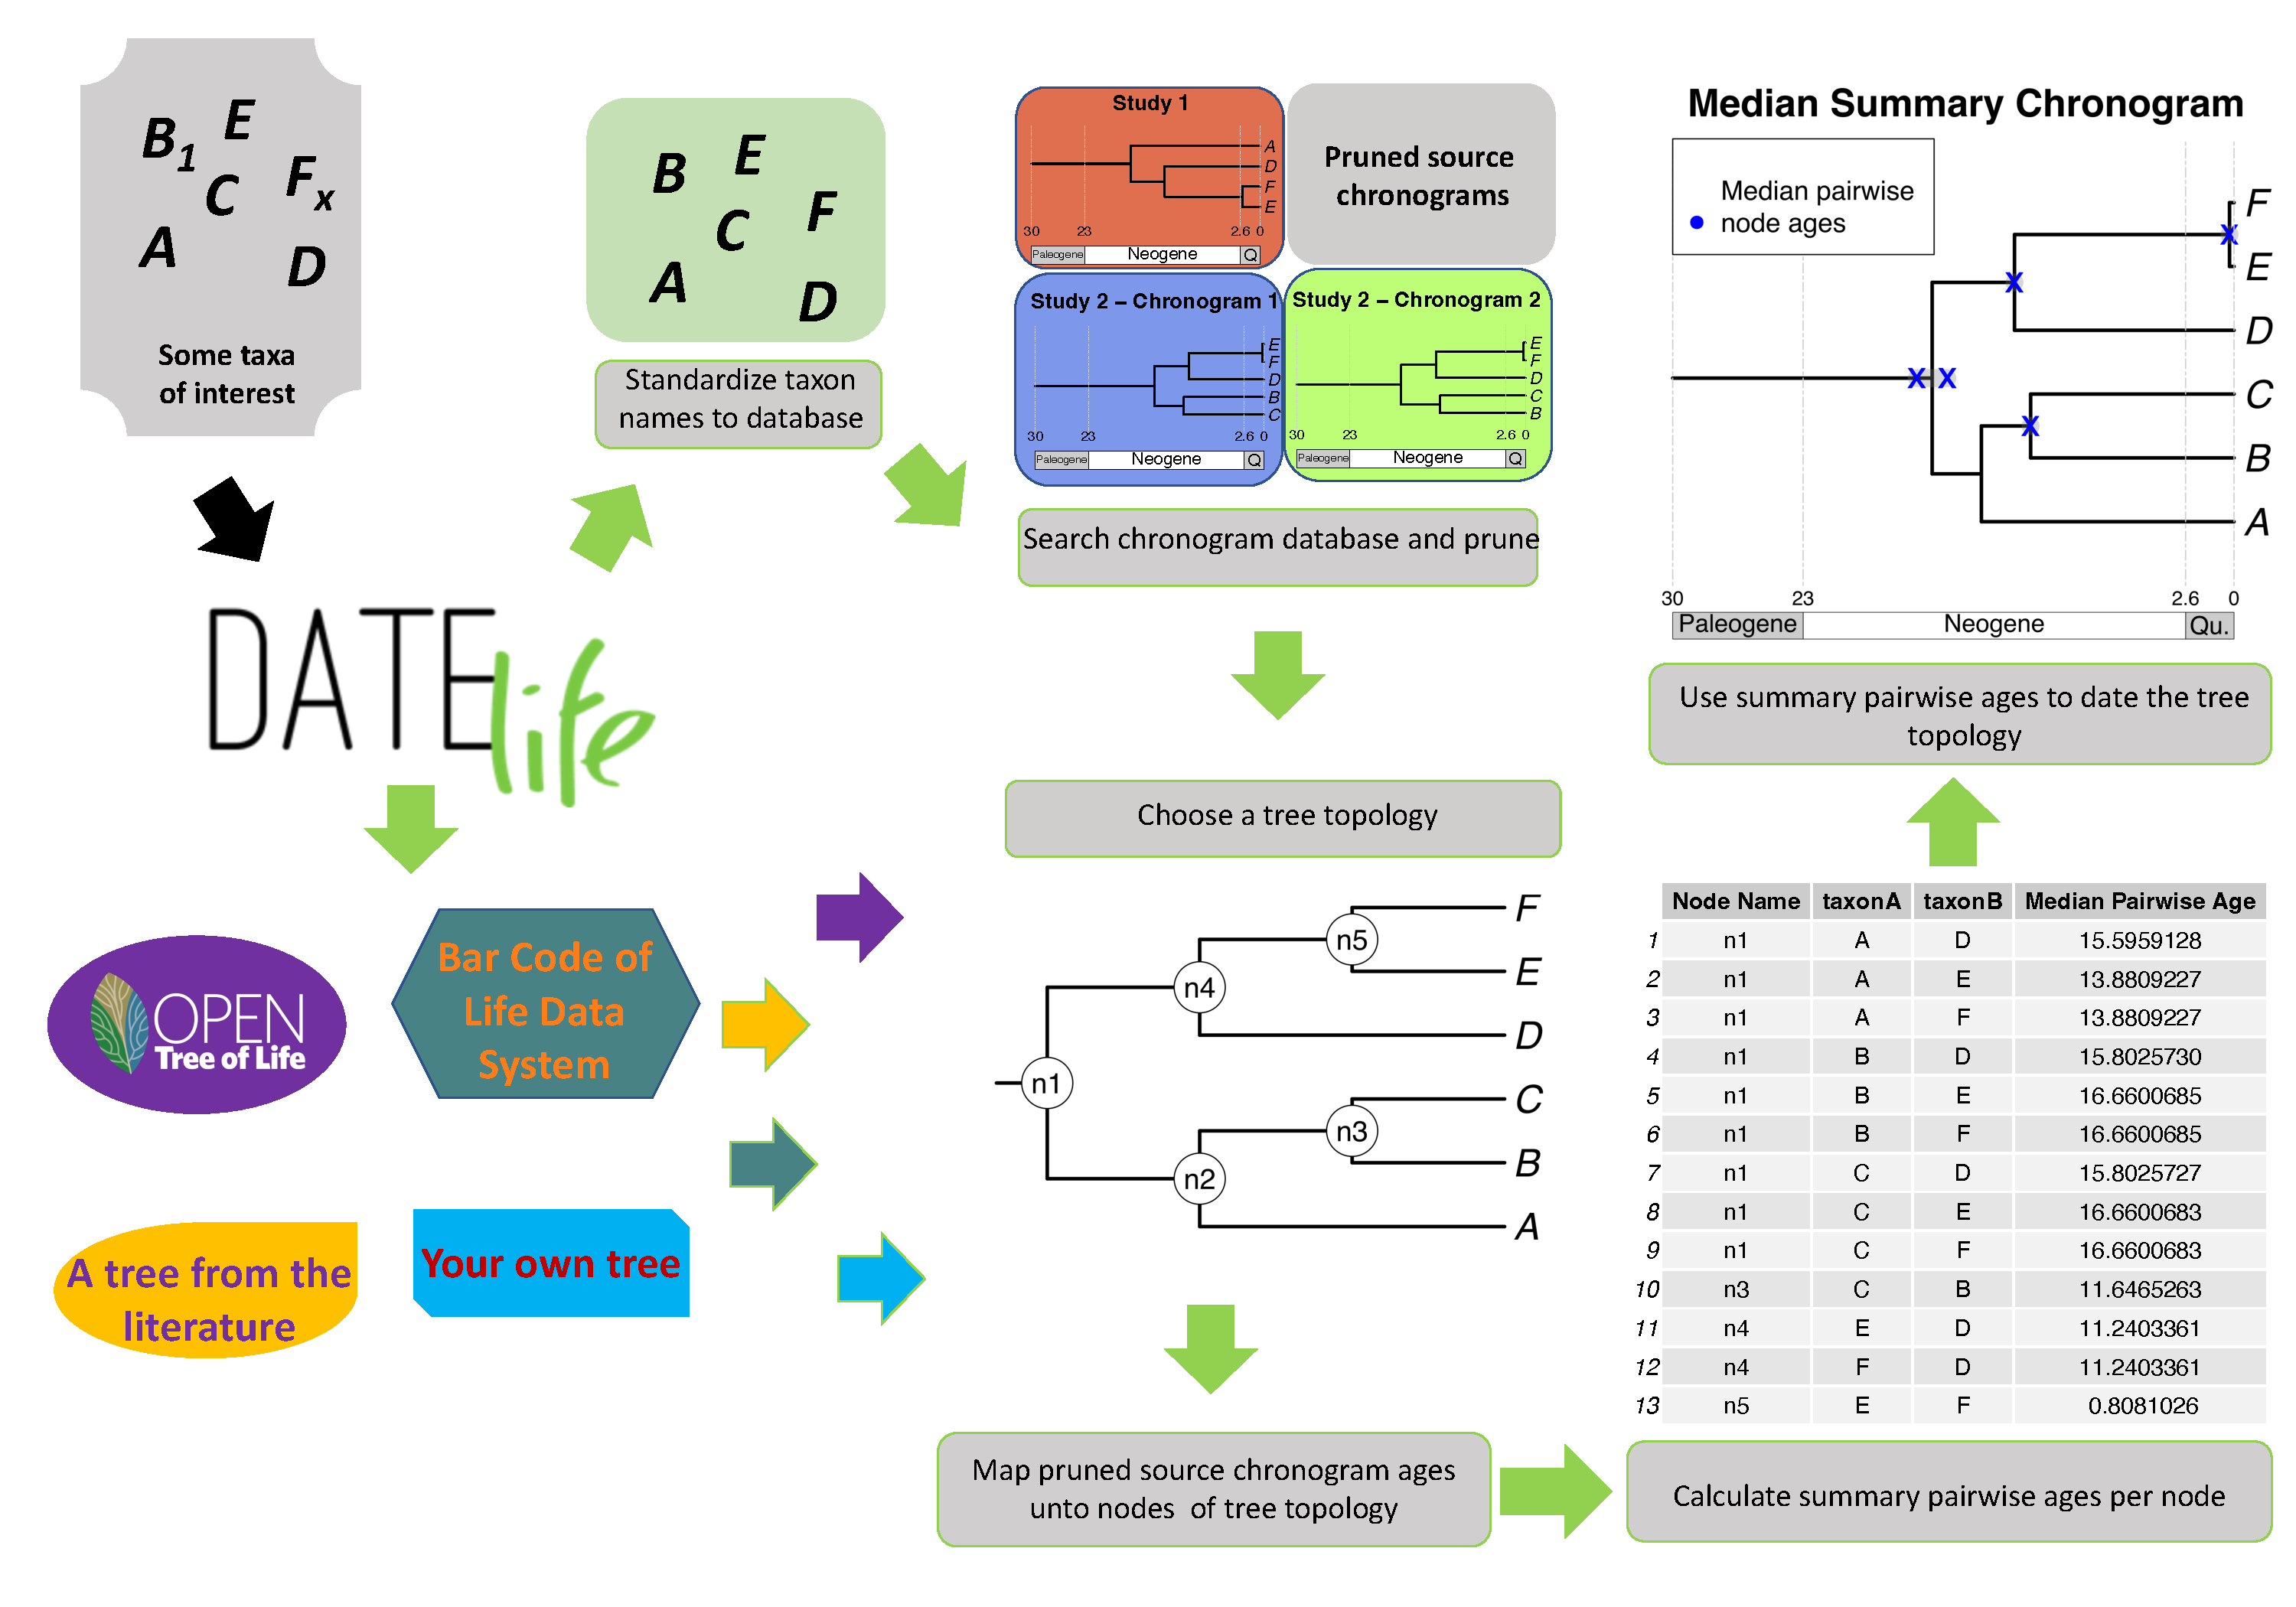
\includegraphics{../figures/figure1/figure1-vertical-final.pdf}
\caption{Stylized DateLife workflow. This shows the general worflows and analyses that can be performed with \texttt{datelife}, via the R package or through the website  at \url{http://www.datelife.org/}. Details on the functions involved on each workflow are shown in \texttt{datelife}'s R package vignette.
}
\label{fig:workflow}
\end{figure}
% \begin{center}
% \textsc{Figure \ref{fig:workflow}}
% \end{center}

\begin{figure}[!h]
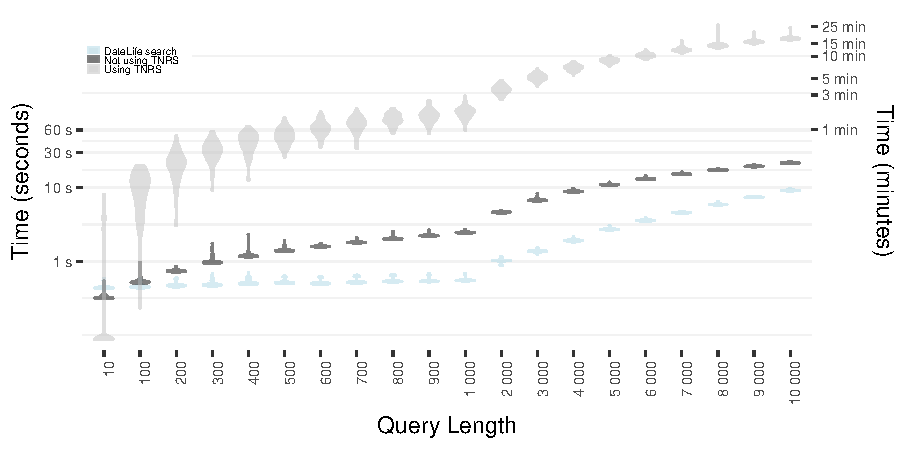
\includegraphics[width=1\linewidth]{../figures/fig_runtime_main.pdf}
\caption{Computation time of query processing and search across \texttt{datelife}'s chronogram database relative to number of input taxon names. We sampled N names from the class Aves for each cohort 100 times and then performed a search with query processing not using the Taxon Names Resoultion Service (TNRS; dark gray), and using TNRS (light gray). We also performed a search using the already processed query for comparison (light blue).}
\label{fig:runtime_main}
\end{figure}
% \begin{center}
% \textsc{Figure \ref{fig:benchmark}}
% \end{center}

\begin{figure}[!h]
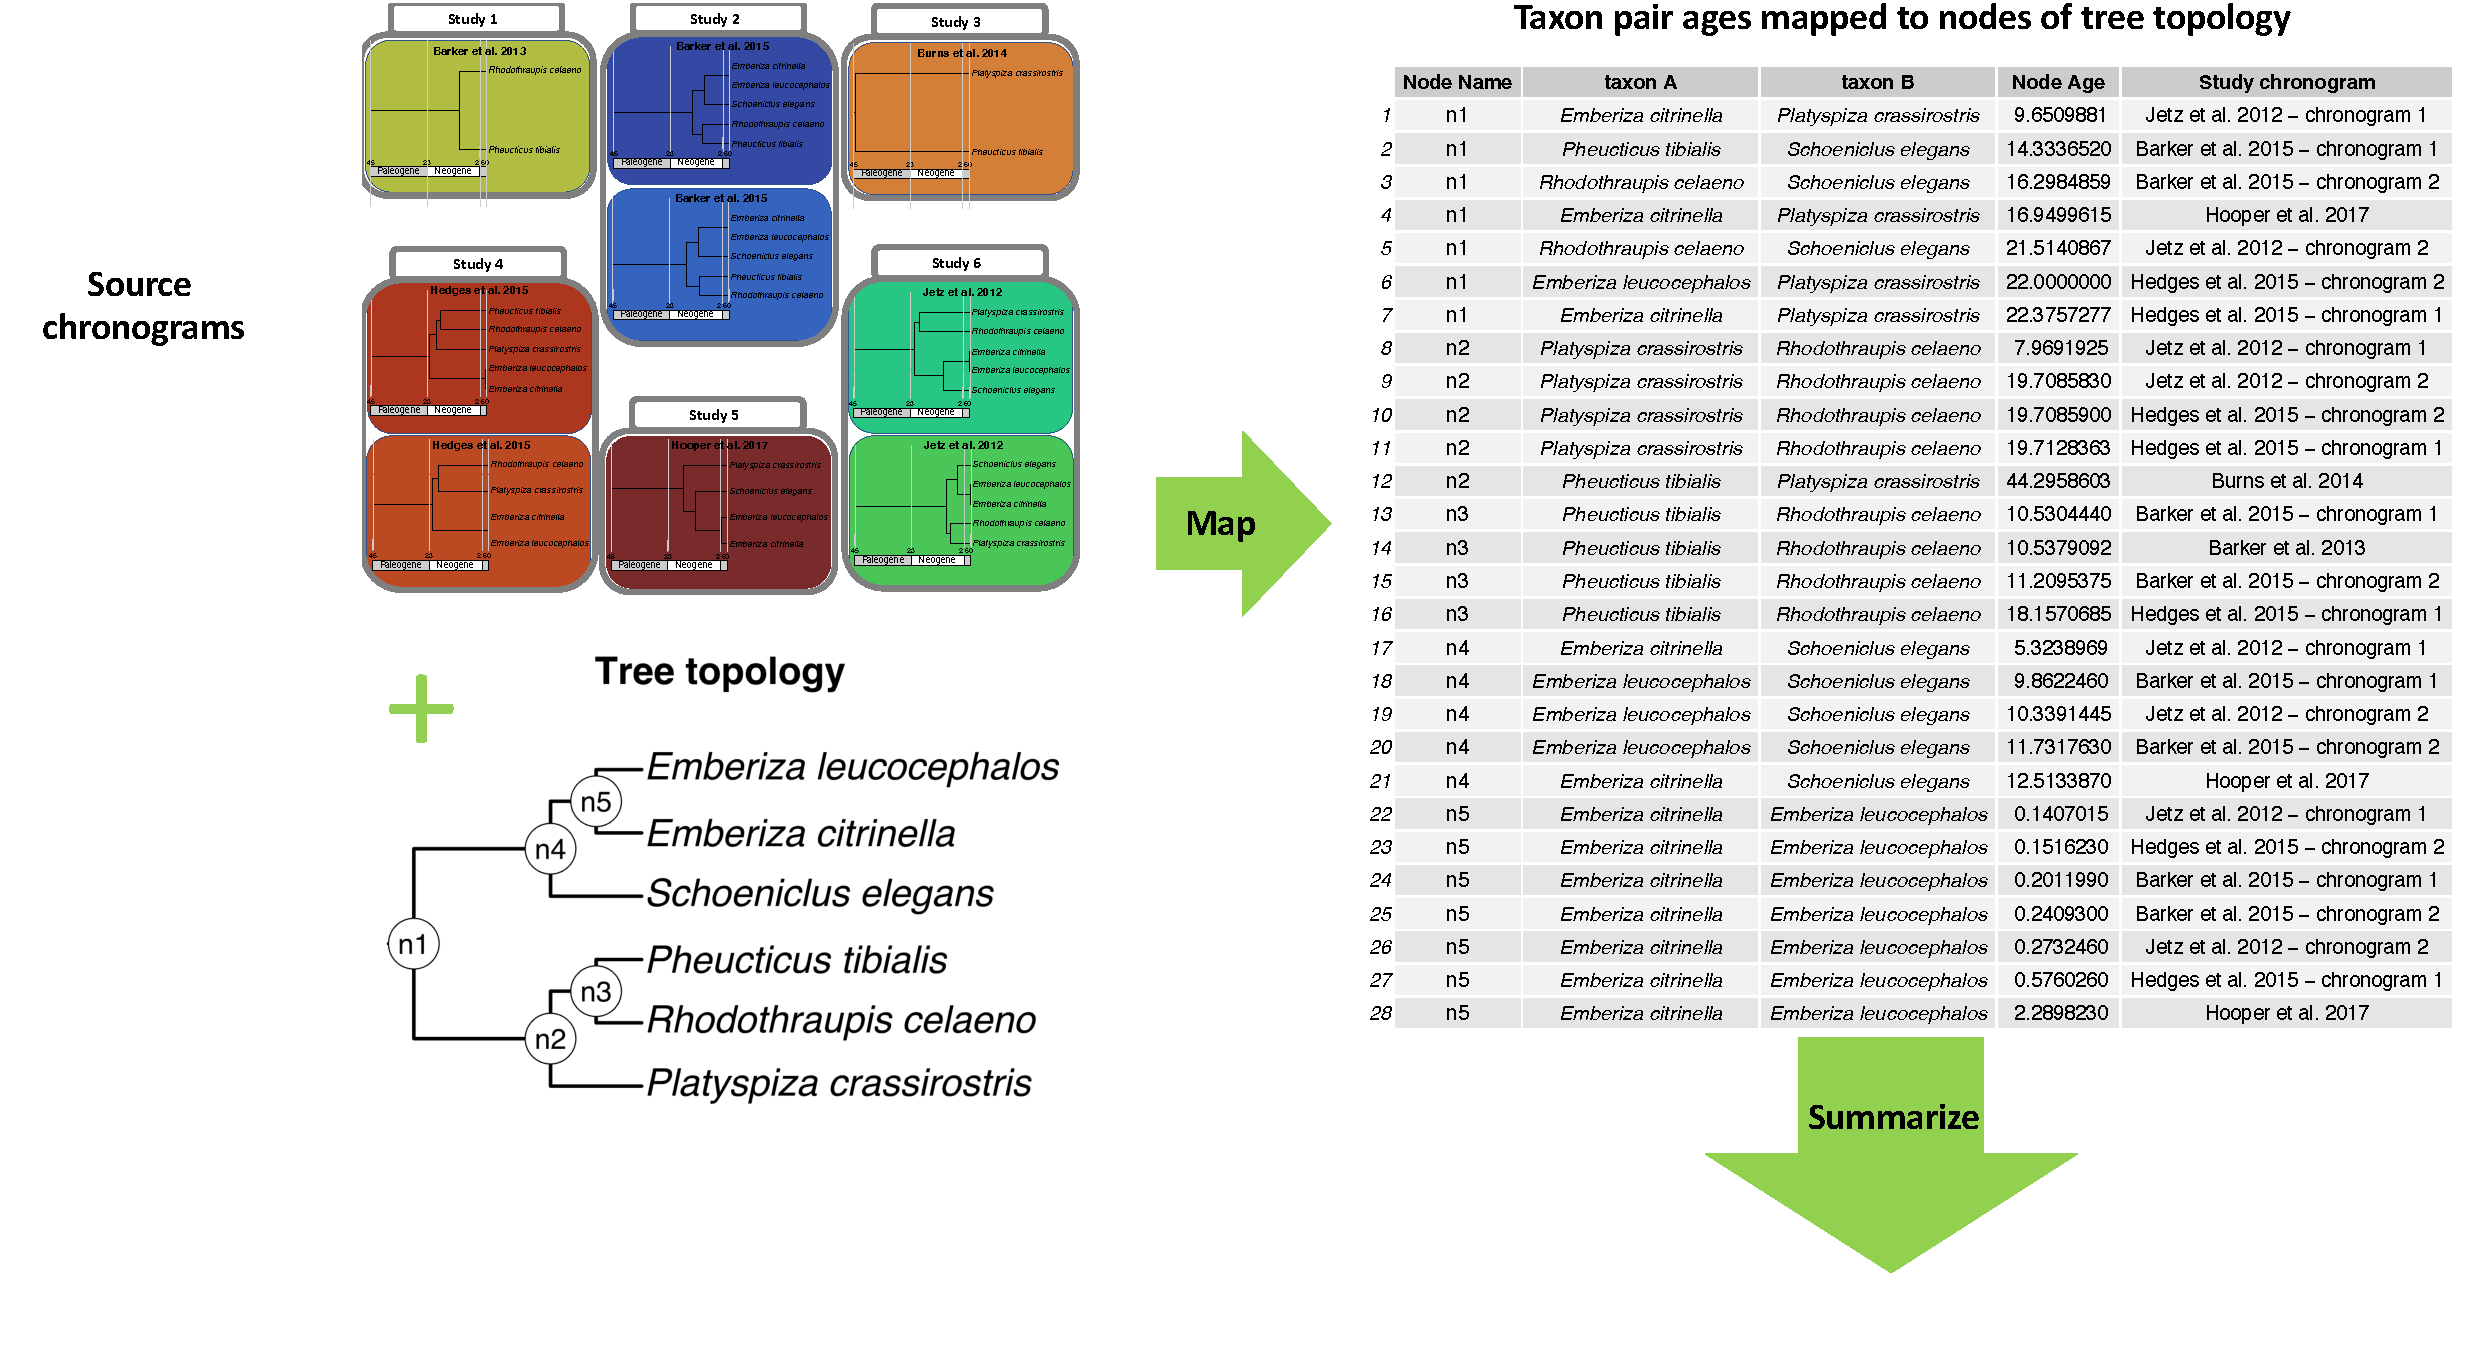
\includegraphics[width=1\linewidth]{../figures/figure2/figure2-1.pdf}
\caption{Age data results of a DateLife search of a small sample of 6 bird species within the Passeriformes. Input names were found across 9 chronograms within 6 independent studies (Barker et al. (\protect\hyperlink{ref-barker2012going}{2012}), Barker et al. (\protect\hyperlink{ref-barker2015new}{2015}), Burns et al. (\protect\hyperlink{ref-burns2014phylogenetics}{2014}), Hedges et al. (\protect\hyperlink{ref-Hedges2015}{2015}), Hooper and Price (\protect\hyperlink{ref-hooper2017chromosomal}{2017}), Jetz et al. (\protect\hyperlink{ref-Jetz2012}{2012}).) This revealed 28 age data points for the queried species names.}
\label{fig:figure2-1}
\end{figure}
% \begin{center}
% \textsc{Figure \ref{fig:figure2-1}}
% \end{center}

\begin{figure}[!h]
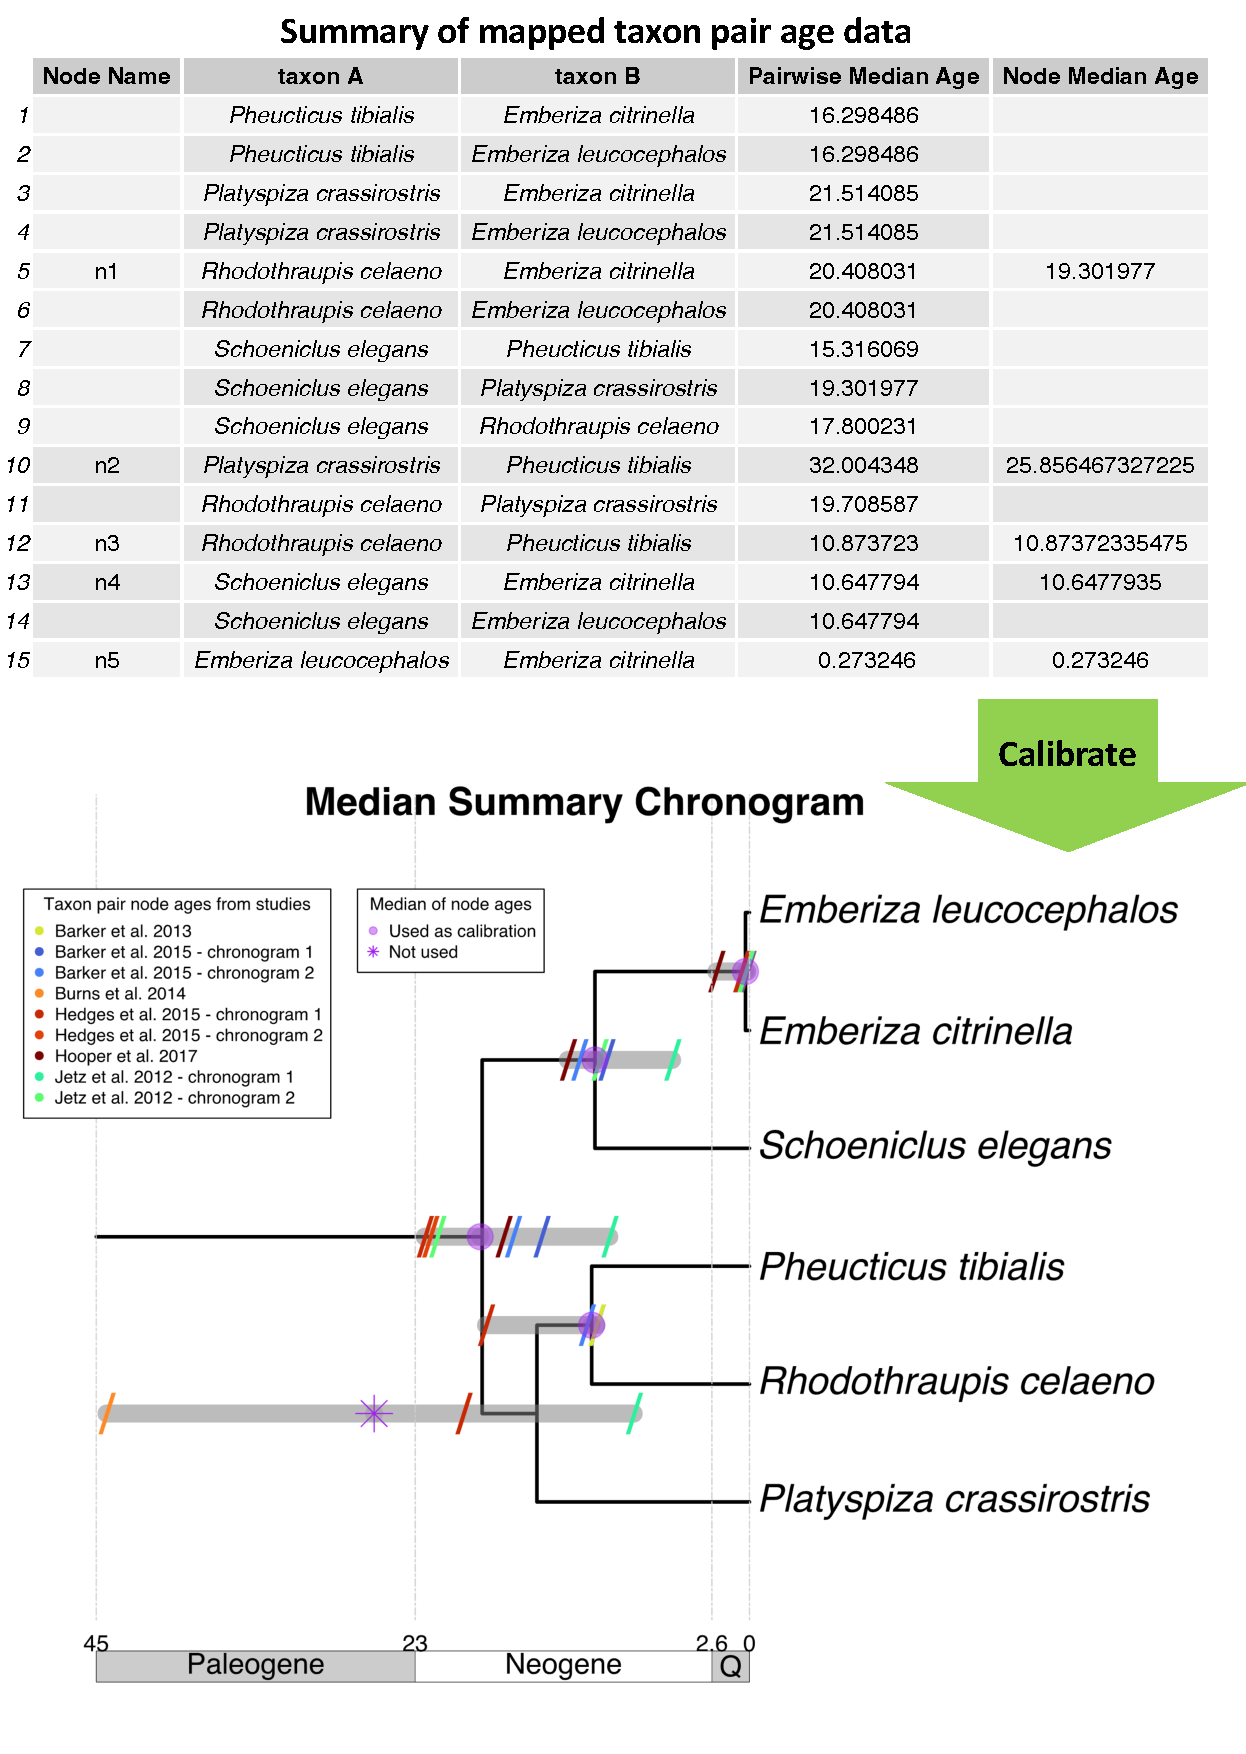
\includegraphics{../figures/figure2/figure2-2.pdf}
\caption{Summarized age data is used as secondary calibrations to date a tree topology as a summary chronogram.}
\label{fig:summaries}
\end{figure}
% \begin{center}
% \textsc{Figure \ref{fig:figure2-2}}
% \end{center}


\begin{figure}[!h]
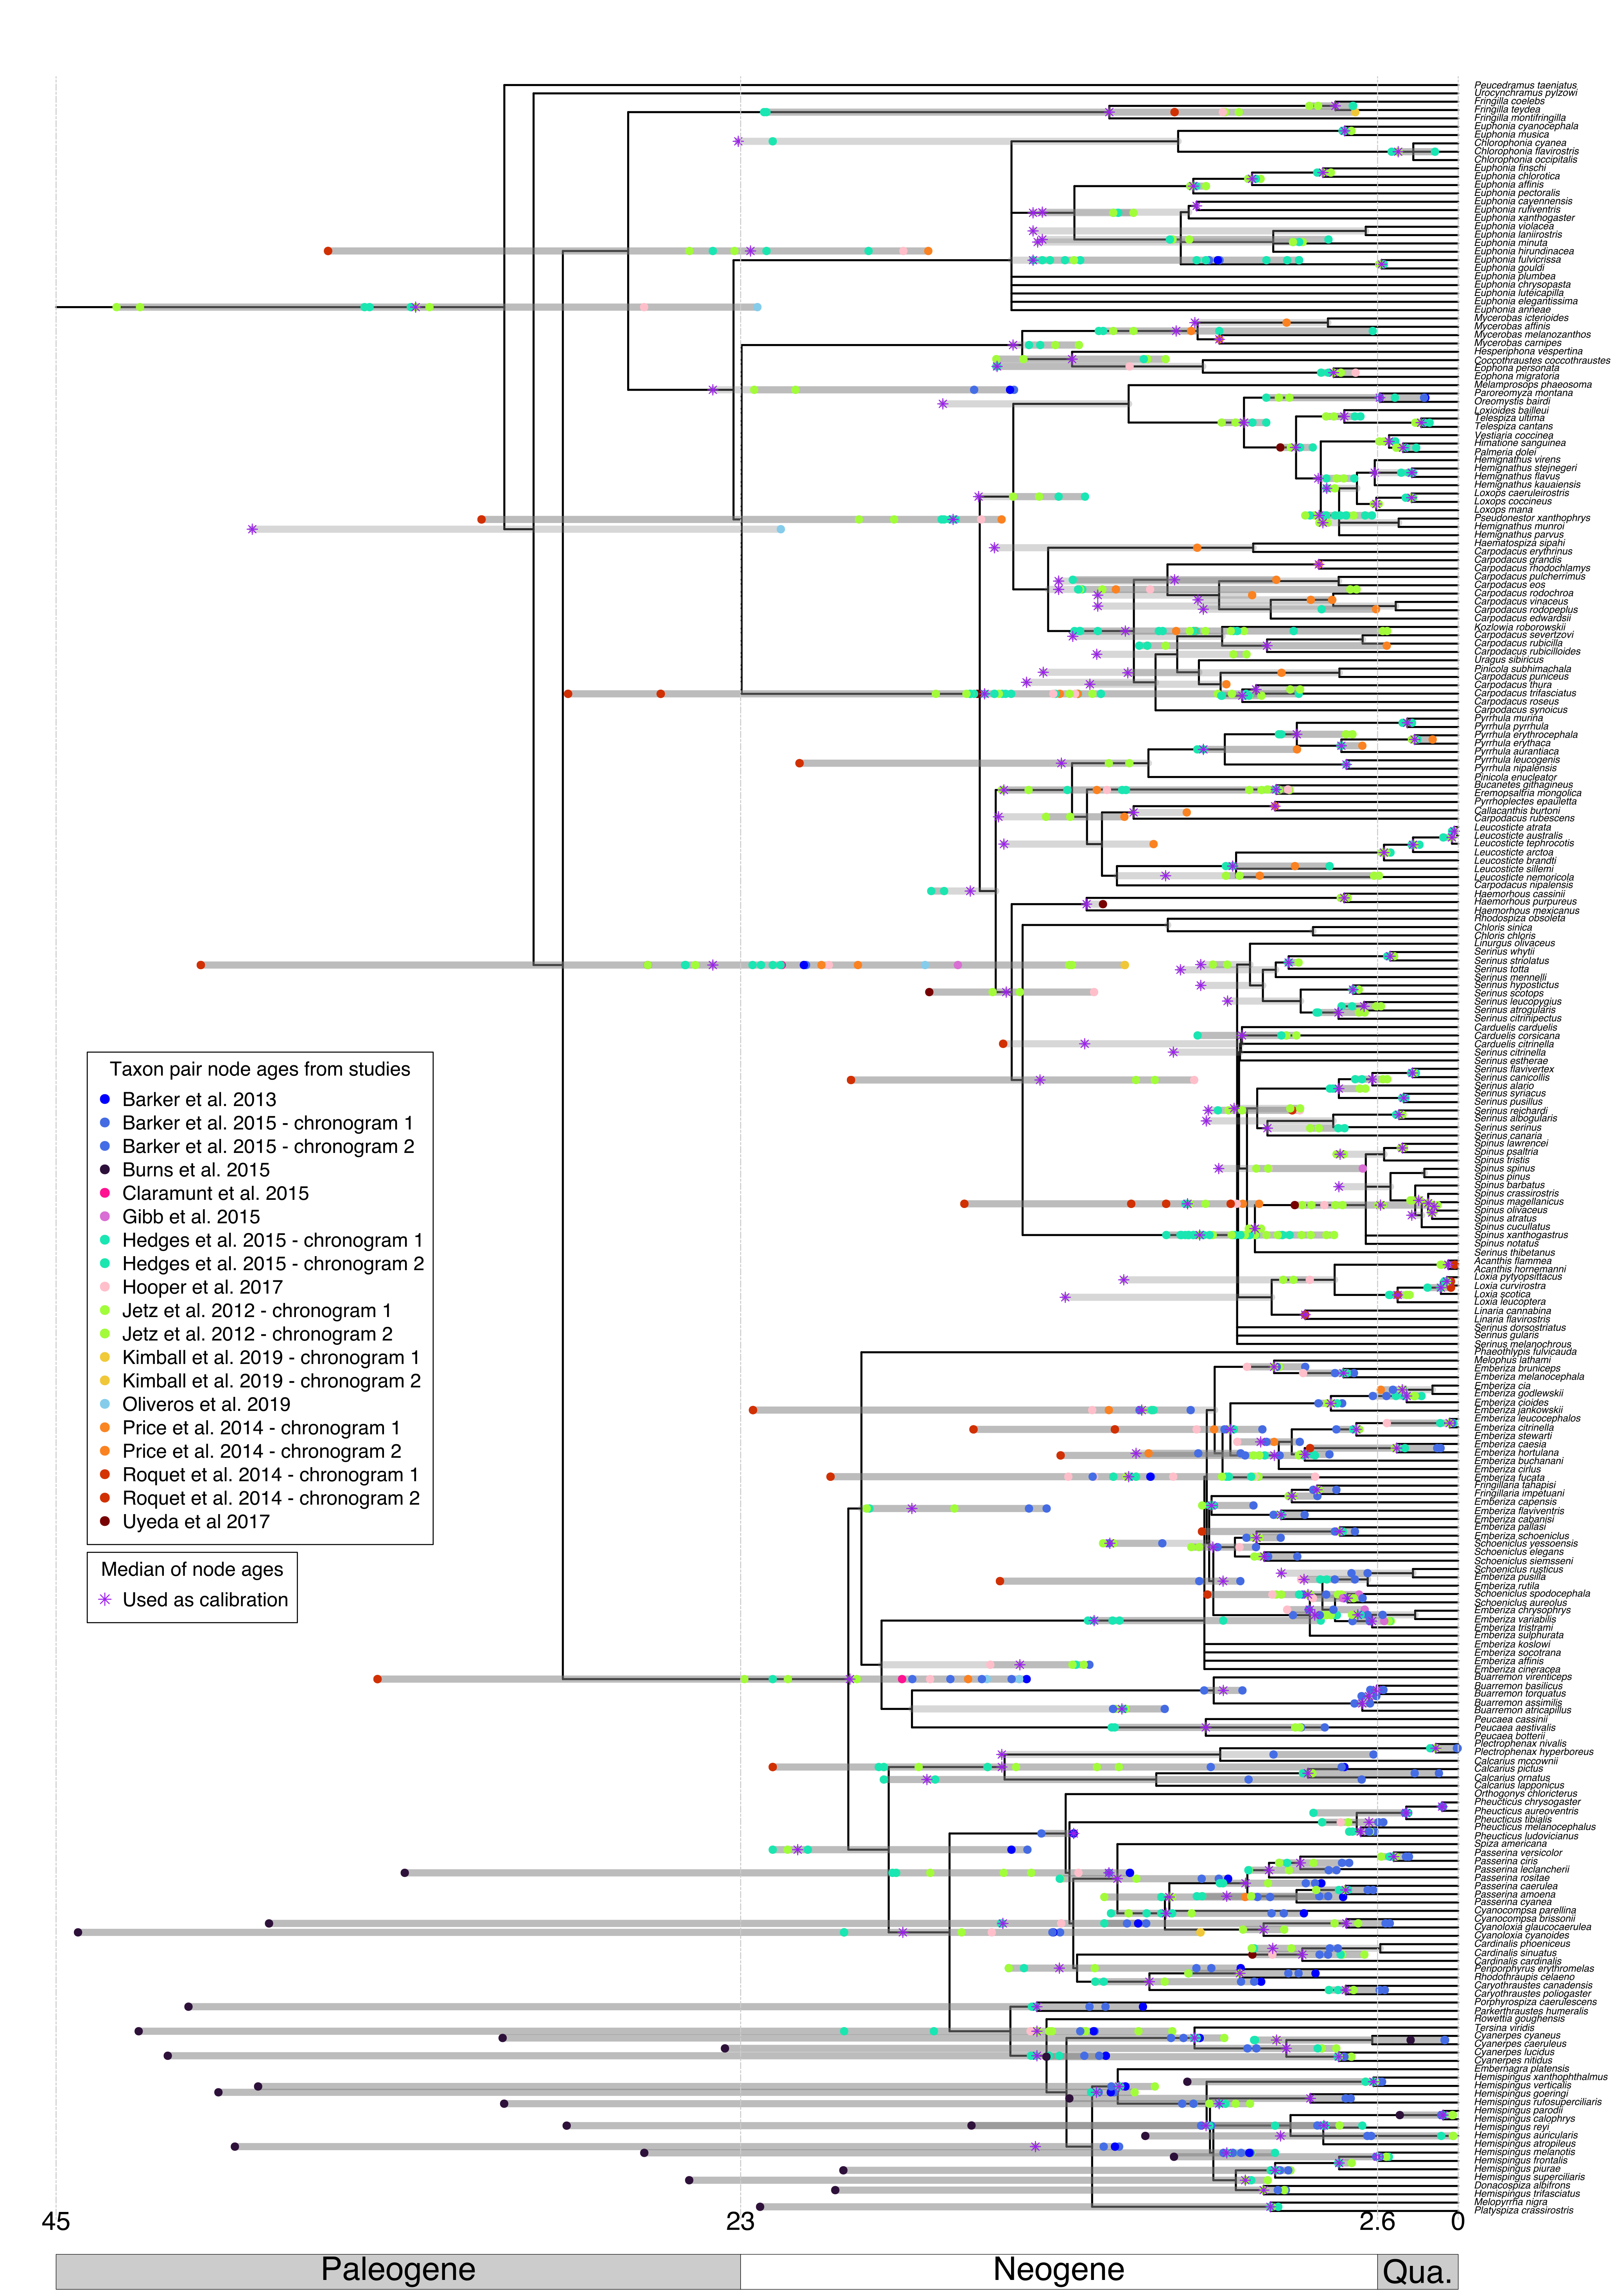
\includegraphics{../figures/figure-fringillidae/median_and_calibration_ages_simple.png}
\caption{Fringillidae median summary chronogram genertaed with DateLife. It has 256 tips and 233 nodes.}
\label{fig:fringillidages}
\end{figure}
% \begin{center}
% \textsc{Figure \ref{fig:fringillidages}}
% \end{center}


\begin{figure}[!h]
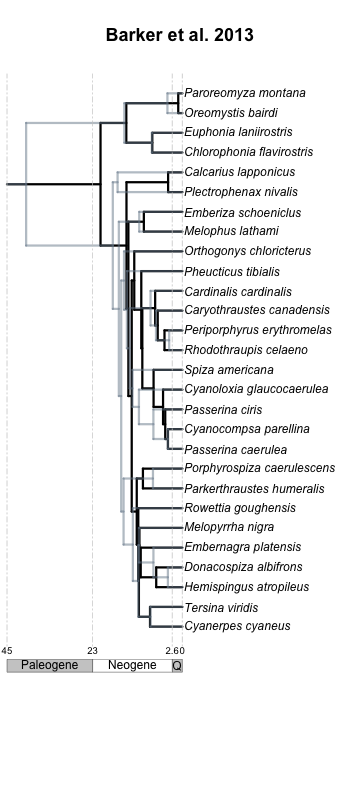
\includegraphics{../figures/figure-cross-validation/cross_validation_1.png}
\caption{Cross validation of first source chronogram. The chronogram shown in black corresponds to the dates published in the original study. The gray chronogram corresponds to the same tree topology dated with BLADJ using node ages from all other source chronograms as secondary calibrations.}
\label{fig:cv1}
\end{figure}
% \begin{center}
% \textsc{Figure \ref{fig:cvbold}}
% \end{center}

\begin{figure}[!h]
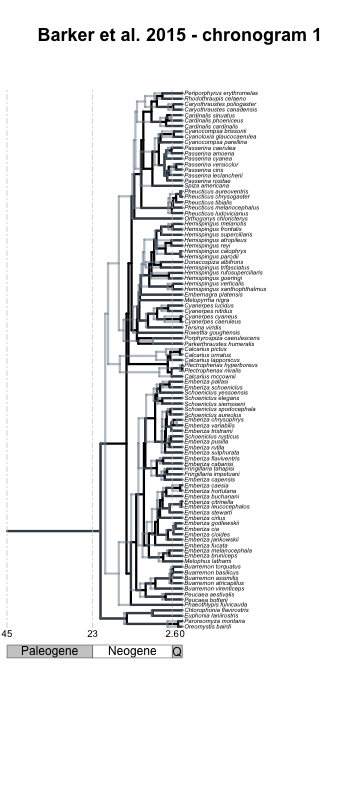
\includegraphics{../figures/figure-cross-validation/cross_validation_2.png}
\caption{Cross validation of second source chronogram. The chronogram shown in black corresponds to the dates published in the original study. The gray chronogram corresponds to the same tree topology dated with BLADJ using node ages from all other source chronograms as secondary calibrations.}
\label{fig:cv2}
\end{figure}

\begin{figure}[!h]
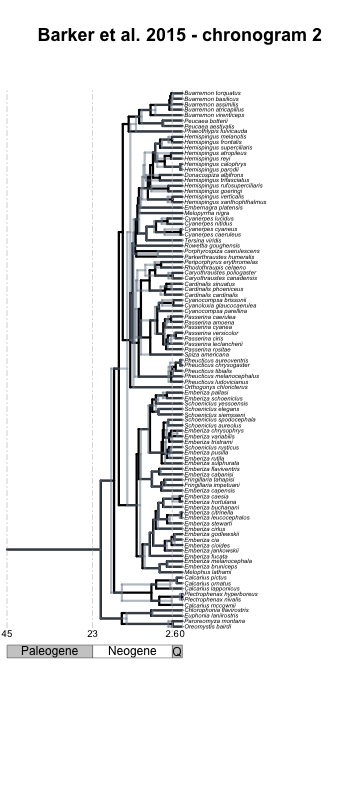
\includegraphics{../figures/figure-cross-validation/cross_validation_3.png}
\caption{Cross validation of third source chronogram. The chronogram shown in black corresponds to the dates published in the original study. The gray chronogram corresponds to the same tree topology dated with BLADJ using node ages from all other source chronograms as secondary calibrations.}
\label{fig:cv3}
\end{figure}

\begin{figure}[!h]
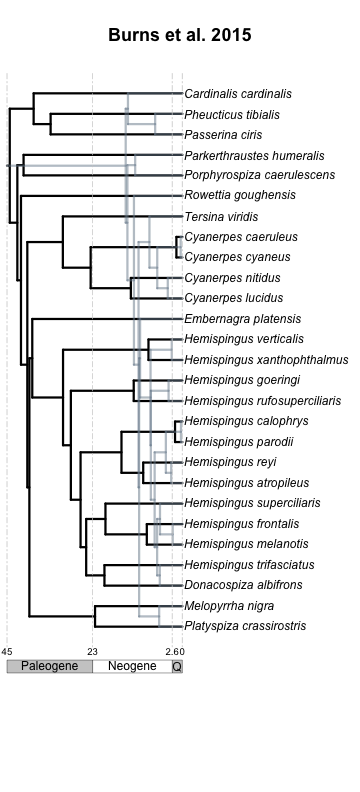
\includegraphics{../figures/figure-cross-validation/cross_validation_4.png}
\caption{Cross validation of fourth source chronogram. The chronogram shown in black corresponds to the dates published in the original study. The gray chronogram corresponds to the same tree topology dated with BLADJ using node ages from all other source chronograms as secondary calibrations.}
\label{fig:cv4}
\end{figure}

\begin{figure}[!h]
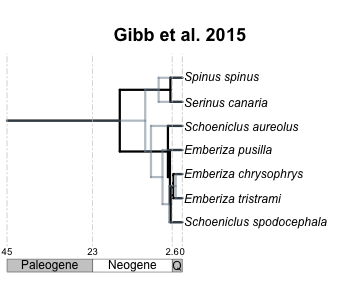
\includegraphics{../figures/figure-cross-validation/cross_validation_6.png}
\caption{Cross validation of sixth source chronogram. The chronogram shown in black corresponds to the dates published in the original study. The gray chronogram corresponds to the same tree topology dated with BLADJ using node ages from all other source chronograms as secondary calibrations.}
\label{fig:cv6}
\end{figure}

\begin{figure}[!h]
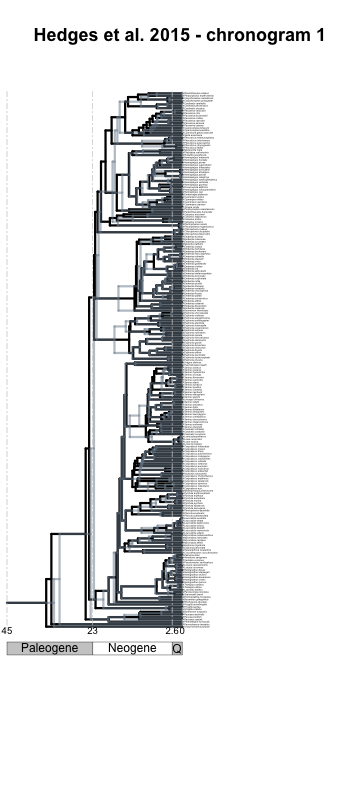
\includegraphics{../figures/figure-cross-validation/cross_validation_7.png}
\caption{Cross validation of seventh source chronogram. The chronogram shown in black corresponds to the dates published in the original study. The gray chronogram corresponds to the same tree topology dated with BLADJ using node ages from all other source chronograms as secondary calibrations.}
\label{fig:cv7}
\end{figure}

\begin{figure}[!h]
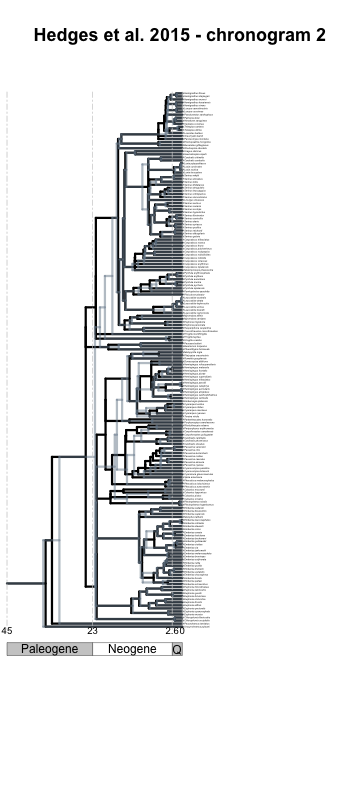
\includegraphics{../figures/figure-cross-validation/cross_validation_8.png}
\caption{Cross validation of eight source chronogram. The chronogram shown in black corresponds to the dates published in the original study. The gray chronogram corresponds to the same tree topology dated with BLADJ using node ages from all other source chronograms as secondary calibrations.}
\label{fig:cv8}
\end{figure}

\begin{figure}[!h]
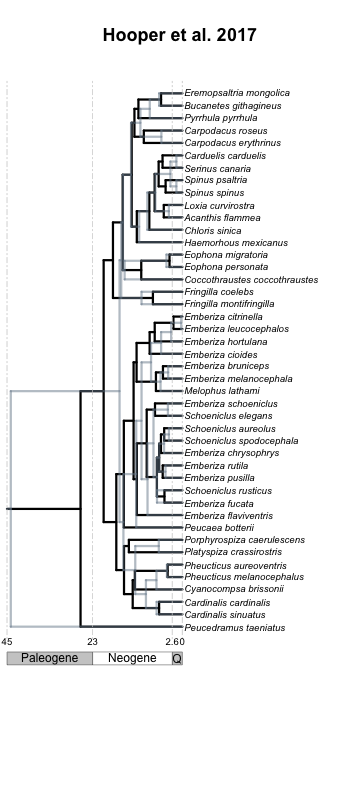
\includegraphics{../figures/figure-cross-validation/cross_validation_9.png}
\caption{Cross validation of ninth source chronogram. The chronogram shown in black corresponds to the dates published in the original study. The gray chronogram corresponds to the same tree topology dated with BLADJ using node ages from all other source chronograms as secondary calibrations.}
\label{fig:cv9}
\end{figure}

\begin{figure}[!h]
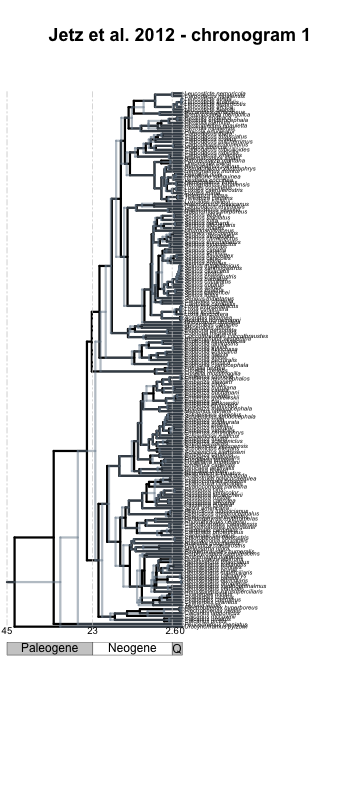
\includegraphics{../figures/figure-cross-validation/cross_validation_10.png}
\caption{Cross validation of tenth source chronogram. The chronogram shown in black corresponds to the dates published in the original study. The gray chronogram corresponds to the same tree topology dated with BLADJ using node ages from all other source chronograms as secondary calibrations.}
\label{fig:cv10}
\end{figure}

% \end{linenumbers}

\end{document}
